\documentclass[11pt,letterpaper]{article}
\usepackage[T1]{fontenc}
\usepackage[utf8]{inputenc}
\usepackage{lmodern}
\usepackage[margin=1.06in,top=.97in,bottom=1.02in,headheight=15pt,headsep=18pt]{geometry}
\usepackage{amsmath,amssymb,amsthm,mathtools,booktabs,array,tabularx,longtable,microtype}
\usepackage{tikz}
\usetikzlibrary{arrows.meta}
\usepackage{xcolor,titlesec,fancyhdr,enumitem,xurl}
\definecolor{ink}{HTML}{183548}
\definecolor{ocean}{HTML}{126C75}
\definecolor{muted}{HTML}{52636B}
\usepackage[colorlinks=true,linkcolor=ocean,urlcolor=ocean,citecolor=ocean,bookmarksnumbered=true,pdfencoding=auto,psdextra]{hyperref}
\hypersetup{bookmarksdepth=2,pdftitle={Theta lifts and the zeros of Dirichlet L-functions},pdfauthor={A synthesis of the ProveIt guide and Ye Yu's exposition}}
\setcounter{tocdepth}{1}
\setlength{\parskip}{3.4pt plus .8pt minus .5pt}
\setlength{\parindent}{1.05em}
\setlength{\emergencystretch}{2.5em}
\raggedbottom
\setlist{itemsep=2pt,topsep=4pt,parsep=1pt}
\titleformat{\section}{\normalfont\Large\bfseries\color{ink}}{\thesection}{.65em}{}
\titleformat{\subsection}{\normalfont\large\bfseries\color{ink}}{\thesubsection}{.55em}{}
\titlespacing*{\section}{0pt}{15pt plus 4pt minus 3pt}{6pt}
\titlespacing*{\subsection}{0pt}{11pt plus 2pt minus 1pt}{4pt}
\pagestyle{fancy}\fancyhf{}
\fancyhead[L]{\small\sffamily\color{muted}Theta lifts and Dirichlet zeros}
\fancyhead[R]{\small\sffamily\color{muted}\thepage}
\renewcommand{\headrulewidth}{.3pt}
\newcommand{\src}[2]{\href{https://github.com/VladimirReshetnikov/ProveIt/blob/7a5bb1e051e4bad127bafe90abbea19764778e32/Analysis/GeneralizedRiemannHypothesis/Lean/grh/#1}{#2}}
\newcommand{\ghout}[2]{\href{https://github.com/sdyy1990/riemann-hypothesis/blob/5edf43ce39c068fec64e0cc122e9cbdcec343b24/#1}{#2}}
\newcommand{\gd}[1]{\href{https://github.com/VladimirReshetnikov/ProveIt/blob/7a5bb1e051e4bad127bafe90abbea19764778e32/Analysis/GeneralizedRiemannHypothesis/docs/guide/theta_lifts_and_dirichlet_zeros.tex}{#1}}
\newcommand{\sources}[1]{\par{\small\color{muted}\noindent\textit{Source.} #1\par}}
\newtheorem{statement}{Theorem}[section]
\newtheorem{proposition}[statement]{Proposition}
\newtheorem{lemma}[statement]{Lemma}
\DeclareMathOperator{\ord}{ord}
\begin{document}
\thispagestyle{empty}
{\small\sffamily\color{ocean} NUMBER THEORY \quad / \quad MATHEMATICAL EXPOSITION}\par
\vspace{.55in}
{\fontsize{31}{36}\selectfont\bfseries\color{ink}Theta lifts and the zeros\\of Dirichlet \(L\)-functions\par}
\vspace{.18in}
{\large A natural-language presentation of the proof of Levent Alpöge with Claude\par}
\vspace{.31in}{\color{ocean}\hrule height 1.1pt}\vspace{.14in}
\noindent\textbf{Abstract.}
Fix a large integer \(x\). An excess in a smoothed count of prime powers makes certain integral automorphic forms unusually short. A chain of about \(\sqrt{x}\) theta lifts repeats the gain. A spanning theorem ensures that enough of the short forms are independent, and a determinant calculation forces their joint squared volume, corrected for denominators, to exceed a precise lower bound. The main terms in the two bounds agree. Their difference gives \(R_Q(x)\le x^{-1/2+\varepsilon}\) eventually for each admissible modulus and quadratic twist. We derive the analytic implication of this one-sided estimate by choosing a twist, identifying the residues of a Mellin transform, and applying Landau's theorem for positive measures. The functional equation then places the zeros on the critical line.
\par\vspace{.12in}
\noindent The exposition combines the ProveIt guide's local calculations with Ye Yu's formulation of the three arithmetic theorems, A, B and C. Links in the text identify where the readable Lean development proves the results used. The mathematical endpoints are ordinary RH and GRH for every Dirichlet character of positive modulus.
\vfill
\noindent{\small\sffamily\color{muted} SOURCE EDITION \quad 27 NOVEMBER 2026}\\[3pt]
{\small ProveIt \texttt{7a5bb1e0}\quad $\cdot$ \quad Ye Yu's outline \texttt{5edf43ce}}
\clearpage
\tableofcontents
\bigskip
\noindent{\sffamily\bfseries\color{ink} Reading routes}\par
\noindent For the implication from prime powers to zeros, read Sections~\ref{sec:opening}, \ref{sec:bridge-closure} and \ref{sec:transform}--\ref{sec:landau}. For the construction of multiplicity, follow the two cutoffs in Section~\ref{sec:bridge-jets} into the upper bound in Section~\ref{sec:bridge-short}, then compare the single-lift calculation in Section~\ref{sec:arithmetic-lower}. Appendix~\ref{sec:worked-guide} gives finite calculations that illustrate these steps.
\clearpage
\section{The theorem and the source of the half power}\label{sec:opening}
For a Dirichlet character \(\chi\) of positive modulus \(q\), extend \(\chi\) periodically to the integers, taking value zero away from integers coprime to \(q\). In \(\Re s>1\) its \(L\)-function is the sum of \(\chi(n)n^{-s}\). Elsewhere \(L(s,\chi)\) denotes its meromorphic continuation. Throughout this article GRH means the generalized Riemann hypothesis for these functions, including characters induced from smaller moduli.

\begin{statement}[Half-plane and critical-line forms]\label{thm:main}
For every such \(\chi\), if \(\Re s>1/2\) and either \(\chi\) is nonprincipal or \(s\ne1\), then \(L(s,\chi)\ne0\). Consequently every zero of \(L(s,\chi)\) in \(0<\Re s<1\) has real part \(1/2\). Every zero of the Riemann zeta function other than the trivial zeros at \(-2,-4,\dots\), with its pole at \(1\) excluded, has real part \(1/2\).
\end{statement}

The half-plane theorem is where the proof does its work. The critical-line statement follows by applying the half-plane theorem to a zero and its reflection for the inverse character. The level-one character gives \(\zeta\). To see where the half power enters the half-plane theorem, it helps to start with an elementary determinant.

Let \(u_1,\ldots,u_n\) be independent columns of an \(n\times n\) integer matrix \(U\). Their Gram determinant satisfies
\[
  1\ \le\ |\det U|^2=\det(U^*U)\ \le\ \prod_{j=1}^n\|u_j\|^2 .
\]
On the left is integrality. On the right is Hadamard's inequality. If a prime divides every entry of one column, dividing that column by the prime preserves integrality and saves \(2\log p\) in its log squared norm. More prime divisibility than expected can now have an observable consequence. If it makes too many independent columns too short, the two inequalities become incompatible.

The columns in the proof are forms on unitary groups. They are obtained from differentiated theta kernels. The kernel derivatives have large archimedean sizes and predictable prime-power divisibilities. Dividing out those divisibilities leaves a log size containing \(-m\mathcal R\), where \(\mathcal R\) measures a prime-power excess and \(m\) counts the lifts in a chain. The determinant lower bound includes the much larger background cost \(H\) of the other derivative directions. Three difficulties distinguish the argument from the integer example. One needs sufficiently many independent columns, one must pay for finite denominators, and one must compute the \emph{same} \(H\) on both sides of the comparison. Coarse bounds that differ by a small fixed proportion of \(H\) would obliterate the desired error.

\begin{center}\small
\renewcommand{\arraystretch}{1.17}
\begin{tabularx}{.97\linewidth}{@{}p{.21\linewidth}X@{}}
\toprule
Result & What is carried into the comparison\\ \midrule
A. Short forms & A spanning supply of integral source forms with short normalized images after the untwisted lift, and a separate bound on the index of finite families of images.\\
B. Enough forms & A small set of translates whose images of the ramified source together cover at least \(1-4/b^2\) of the target dimension.\\
C. Long forms & For any independent family that large, its log squared covolume plus twice its denominator allowance is bounded below in terms of \(H\).\\ \bottomrule
\end{tabularx}
\end{center}
The factor of two in C can already be read off from \(U^*U\). A change of basis multiplies a Gram determinant by the product of a determinant and its conjugate. The near-full dimension in B matters twice. It lets us compare an upper bound on actual columns to a lower bound on volume, and it limits how many auxiliary forms C must add to obtain a square determinant.

One might try to get the half power from a square-root cancellation estimate for primes. Here the square root first enters as an integer we choose. For every large \(x\) we can build a chain of \(m\) lifts, \(\sqrt x\le m\le2\sqrt x\). Its upper bound accumulates the same prime excess \(m\) times. Its lower bound pays for the ordinary directions of all \(m\) lifts, up to a loss which, after division by the relevant dimension and weight, grows only as a power of \(\log b\). The scales give \(\log b\le2x^\eta\) for any fixed sufficiently small \(\eta>0\). The resulting \(1/m\) survives in the final estimate.

There are two different uses of twisting. Inside C one chooses finite-order characters of a unitary group, separately at finite coefficient places, to bound denominators and determinant ratios. At the end one chooses a quadratic Dirichlet character depending on a putative zero to isolate the pole it would produce. They have different moduli, different quantifiers, and different effects on the proof.
\sources{\src{src/Statements.lean}{Public statements}, \src{src/Main.lean}{five exported theorems}, \src{src/New/Reduction/MainInequality.lean}{comparison}, and \src{src/New/Reduction/Zeros/Criterion.lean}{one-sided criterion}.}

\subsection{The arithmetic observable}\label{sec:observable}
Fix a positive modulus \(Q\) divisible by \(18480\) and a prime \(d\equiv Q/2-1\pmod Q\). Thus \(d\equiv7\pmod8\) and \((d,Q)=1\). Write \(\chi_d(n)=(n/d)\) for the quadratic character of \(K=\mathbb Q(\sqrt{-d})\). For \(q=Q\) or \(1\) put
\[
 \lambda_{d,q}(n)=\mathbf1_{n\equiv1\bmod q}\,\Lambda(n)(1-\chi_d(n)),\qquad
 R_q(y)=\sum_{n\le y}\lambda_{d,q}(n)
 \left(\frac1n-\frac1y\right)-\frac{\log y}{\varphi(q)}-c_q.
\]
Here \(\Lambda(p^e)=\log p\) for \(e\ge1\) and is zero elsewhere. At a split prime the weight vanishes. At an inert prime it is \(2\log p\) at odd powers and zero at even powers, subject in each case to the congruence on the \emph{power}. At the ramified prime \(d\) it is \(\log d\) at every power allowed by the congruence. The constants \(c_q\) are fixed below by an analytic regularization. This is important because an arbitrary additive constant would be larger than the upper bound we intend to prove.

Let \(E_\psi(s)\) be \(L(s,\psi)\) for a nonprincipal character and the entire continuation of \((s-1)L(s,\psi)\) for a principal character. Define
\begin{equation}\label{eq:Gmean}
 G_q(s)=\frac1{\varphi(q)}
 \left[\sum_{\psi\bmod q}
 \left(\frac{E'_{\psi\chi_d}}{E_{\psi\chi_d}}(s)
       -\frac{E'_\psi}{E_\psi}(s)\right)-1\right],
 \qquad c_q=\Re G_q(1).
\end{equation}
The character sum commutes with complex conjugation on the real axis, so \(G_q(1)\) is real. The principal character has been regularized and no twist is principal. Logarithmically differentiating the Euler products, and summing characters to pick out the residue \(1\), yields
\[
   \sum_{n\ge1}\frac{\lambda_{d,q}(n)}{n^s}
        =\frac{s}{\varphi(q)(s-1)}+G_q(s) \qquad(\Re s>1).
\]
In particular, for \(Z(s)=(s-1)\zeta(s)\) one has \(Z(1)=1\), \(Z'(1)=\gamma\), and
\[
                c_1=-1-\gamma+\Re\frac{L'}{L}(1,\chi_d).
\]
An elliptic period in the construction will recover exactly this constant. The remaining sections prove that for each fixed \(Q,d\) and every \(\varepsilon>0\),
\begin{equation}\label{eq:target}
                R_Q(y)\le y^{-1/2+\varepsilon}
                \qquad\hbox{for all sufficiently large real }y.
\end{equation}
Only an upper bound appears here. A negative discrepancy can make an arithmetic vector longer and does not lead to a determinant contradiction. Section~\ref{sec:landau} shows why this is the correct direction for excluding zeros.
\sources{\src{src/New/Reduction/Zeros/PrimeError.lean}{Weights, regularization and Dirichlet series}, \src{src/New/Reduction/OneSidedBound.lean}{eventual real-variable estimate}.}

\section{Constructing the arithmetic data at a prescribed scale}\label{sec:setup}
The proof must bound \(R_Q(x)\) at every sufficiently large \(x\), while using level primes and CM fields with special properties. It achieves this by prescribing a sufficiently large integer \(x\) first. The auxiliary levels, degrees and weights may then depend on it. In this section \(Q,d\), and a small positive \(\eta<1/100\) are fixed.

\subsection{A field whose places can detect a progression}
Take \(m\) to be the least power of two at least \(\sqrt{x}\), and \(r\) the least power of three at least \(x^5\). Then \(m\le2\sqrt{x}\) and \(r\le3x^5\). Put \(k=r+1-m\), \(t=5r\), and choose the integer \(s_0\) with \(2^{s_0}=m^{22}\). If \(l_0\) is the least power of three strictly larger than \(27s_0\), set
\[
 T_0=3l_0\,2^{s_0},\qquad q_1=QT_0,\qquad q_2=(Qd)^{s_0+6},
 \qquad E=K(\zeta_{q_1}).
\]
Complex conjugation gives the CM field \(E\) its totally real fixed field \(E^+\). Choose one of the embeddings of \(K\) into \(\mathbb C\). Each conjugate pair of embeddings of \(E\) now has a distinguished member, the one extending that embedding of \(K\). The coprime quadratic and cyclotomic conductors make the possible images of \(\zeta_{q_1}\) exactly its powers by the units modulo \(q_1\). Hence the infinite places \(\Phi\) carry the group structure of \((\mathbb Z/q_1\mathbb Z)^\times\). Write \(f=|\Phi|\).

Let \(\Phi_a\) be the whole fibre above \(1\) modulo \(Q\), and let \(\Phi_b\) be a carefully chosen subset of the fibre above \(-1\). Reduction modulo \(Q\) has equal-size fibres. The prime divisors of \(T_0\) already divide \(Q\), so
\[
             |\Phi_a|=T_0,\qquad f=\varphi(Q)|\Phi_a|.
\]
Put \(W=x^{\eta/6}\), \(x_1=\lfloor e^W\rfloor\), and choose \(b\) as the least multiple of \(q_1x_1\) strictly exceeding \(e^{W^6}\). With \(a=xb\), the inequalities
\[
       x^\eta\le\log b\le x^\eta+1,\qquad
       x^{\eta/6}-1\le\log x_1\le x^{\eta/6}
\]
hold eventually. Each place carries an ordinary integral weight
\[
 \kappa(\tau)=
 \begin{cases}b=a/x,&\tau\in\Phi_b,\\ a/x_1,&\tau\notin\Phi_b.\end{cases}
\]
At the places in \(\Phi_a\) we also use a distinguished derivative of order \(a\). Thus a place in \(\Phi_a\) has ordinary weight \(a/x_1\) as well as the extra long derivative. The translates of \(\Phi_b\) will determine which of two cutoffs this derivative measures.

To see the selection rule in a small group, reduce the units modulo \(21\) to the units modulo \(3\). The \(+1\) fibre is \(A=\{1,4,10,13,16,19\}\). Mark \(B=\{2,11\}\) in the \(-1\) fibre. At \(n=13\), multiplication by \(-n\) sends \(A\) onto the \(-1\) fibre, so exactly two of the six partners are marked. At \(n=5\), the same multiplication sends \(A\) onto itself, so none are marked. This is the only group fact needed for the progression selector. In the actual field all prime powers with nonzero weight are units modulo \(q_1\), since the prime divisors of \(q_1\) split in \(K\). Applying the selection rule to the positive part
\[
       (a/n-\kappa(-n\tau))_+
       =a(1/n-1/x)_+\quad\hbox{or}\quad a(1/n-1/x_1)_+
\]
shows how a sum of derivative valuations distinguishes the residue \(1\bmod Q\).
\sources{\src{src/New/Reduction/Data/FieldsAndPlaces.lean}{Fields, embeddings and place classes}, \src{src/New/Reduction/Data/AdmissibleData.lean}{data and weights}, \src{src/New/Reduction/PrimeSums.lean}{the fibre count}.}

\subsection{Density and sparsity of the marked places}
If \(B=\Phi_b\) were very small, the term involving \(R_Q(x)\) would be swamped when we divide a total excess by \(a|B|\). On the other hand, clusters of large weights at places related by small prime powers would destroy a bound for simultaneous local divisibility. The construction proves both
\[
        |B|\log b\ge|\Phi_a|
\]
and the following restriction. For every prime \(\ell\le kt\) and \(0<i<j<l_0\), there are no \(\sigma,\tau,\rho\in B\) and independent signs such that
\[
 \tau/\sigma\equiv\pm\ell^i,\qquad
 \rho/\sigma\equiv\pm\ell^j
 \pmod{\text{prime-to-}\ell\text{ part of }q_1}.
\]
Even repeated places are covered by this restriction.

The geometric ingredient is a sphere of integer digit vectors. Partition the vectors in \(\{0,\ldots,h-1\}^{v}\) by squared length. One sphere contains at least \(h^v/(vh^2)\) vectors for positive \(h,v\). Encode their digits in base \(Lh\), with modulus \(o\ge(Lh)^v\). A relation
\((u+v')e_2\equiv u e_1+v'e_3\pmod o\), with \(u,v'>0\) and \(u+v'\le L\), is an equality digit by digit. The base prevents carries and the modulus prevents wraparound. After division by \(u+v'\), the middle vector is a convex combination of two vectors of the same squared length as itself. The strict convexity of squared length forces all three vectors to coincide.

Here the exponents \(e\) label places with unit class \(-g^e\), where \(g=1+3l_0Q\). On the indicated power-of-two component of the modulus \(g\) has order \(2^{s_0}\). For odd \(\ell\), raising two hypothetical prime-power congruences to powers \(2j\) and \(2i\) removes their signs and produces the same \(\ell^{2ij}\). The resulting congruence for the three exponents has coefficients \(2(j-i),2i\) and sum \(2j\le2l_0\). The digit lemma forces equality of the exponents. The remaining order condition would imply \(2^{s_0}\le2i(\ell+1)\), which the construction prevents by \(2l_0(kt+1)<2^{s_0}\). For \(\ell=2\) the odd part of the modulus still contains \(3l_0\), and the order of \(4\) there excludes the two relations. The resulting set satisfies \(|B|\ge T_0/W^6\). Since \(W^6\le\log b\), it is sufficient even after all the exclusions.
\sources{\src{src/New/Reduction/Data/Existence.lean}{Sphere lemma, multiplicative orders and existence of sparse places}.}

\subsection{Levels, periods and the two chains of spaces}
Two primes \(p_0,p_1\in[b^{10},b^{11}]\), both \(1\bmod q_2^2\), give \(M=p_0p_1\). We need to write \(M\) as the norm of an algebraic integer in \(K\). One split prime by itself can represent a nontrivial ideal class. Take \(h_K+1\) distinct split primes in admissible windows, where \(h_K\) is the class number, and choose one prime ideal above each. Two selected ideals \(I_i,I_j\) have the same class. Then \(I_i\overline{I_j}\) is principal, and its generator has norm \(p_ip_j\). This supplies the required pair.

A further prime \(N\equiv1\bmod q_2^2\) lies in the window
\begin{align}
 \log N_-&=m\log\bar\kappa+(m-1)\log\!\left(\frac{M\,\mathrm{rd}_E}{2\pi}\right)
                       -\tfrac{15}{2}\log b,\label{eq:Nlevel}\\[-2pt]
 \log N_-&\le\log N\le\log N_-+\sqrt{\log b},\qquad
 \log\bar\kappa=f^{-1}\sum_{\tau\in\Phi}\log\kappa(\tau).\notag
\end{align}
Here \(\mathrm{rd}_E\) is the root discriminant of \(E\). The size of the levels relative to the progression modulus permits the use of prime windows of Siegel--Walfisz type. Also \(i=\sqrt{-1}\in E\) and \(N\equiv1\bmod4\), so a representation \(N=u^2+v^2\) gives \(\pi_N=u+iv\) with \(\pi_N\overline{\pi_N}=N\). The order of these choices matters. The marked places determine \(\bar\kappa\), and both \(\bar\kappa\) and the previously chosen \(M\) determine the window for \(N\).

We explain why the leading terms in \eqref{eq:Nlevel} have these coefficients. The cost of a derivative of order \(h\) at infinity is
\(s_\infty(h)=\log h!+h\log(M/\Omega)\), with
\[
 \Omega=\frac{2\pi}{\mathrm{rd}_E}
   \exp\!\left(\gamma-\Re\frac{L'}{L}(1,\chi_d)\right).
\]
The Chowla--Selberg formula supplies the normalization of the periods of the CM elliptic curves used for the theta series. The source first controls all conjugate periods by a simultaneous scaling which is a unit at every finite place. This lets the same Taylor expansion have the asserted archimedean size and the requisite finite-place divisibility. Thus \(\Omega\) is tied to the derivatives of an actual function. Its relation to \(c_1\) implies
\[
  \log(M/\Omega)=1+c_1+\log(M\,\mathrm{rd}_E/2\pi).
\]
Subtracting the expected finite gain \(a(\log(a/\bar\kappa)+c_1)\) from \(s_\infty(a)\), Stirling's \( -a\) cancels the \(+a\) in the period term. This leaves \(a\log(\bar\kappa M\,\mathrm{rd}_E/2\pi)+O(\log a)\). On the entire chain the final restriction contributes a leading \(-a\log N\) per long place. Formula~\eqref{eq:Nlevel} lets a single restriction repay \(m\) of the leading terms to within \(O(a\log b)\). This explains why an error of fixed size in \(c_1\) would be serious. It would accumulate \(m\) times alongside the signal.

The geometric maps are built on two sequences of Hermitian spaces. With \(0\le j\le m\), the definite spaces \(X_j\) have rank \(k+j(t+1)\). The spaces \(Y_j\) have rank \(r+jt\). Initially \(Y_0\) is \(X_0\) together with \((m-2)/2\) hyperbolic planes and one line of norm \(-N\). At the far end \(Y_m\) is a definite codimension-one subspace of \(X_m\), since \(k+m-r=1\). The integral source forms live on the definite group of \(X_0\). The target being spanned consists of selected forms on \(Y_0\); the norm for such a form is measured after lifting along the \(Y\)-chain to \(Y_m\). This creates two paths to the same terminal calculation. An iterated seesaw identity relates the paths.

At the finite coefficient places a target vector has to meet several tests at once. For a prime \(\ell\) and an identification of the coefficients with \(\overline{\mathbb Q}_\ell\), take the intersection of the inverse images of the integral lattices under all admissible lifts \(\Theta_\xi\) of conductor prime to \(\ell\). A bound \(\delta\) on the index of a family \(y_i\) means that at each such identification there is an integral matrix \(U\) taking the tuple into this intersection, with \(|\det U|_\ell\ge\ell^{-e_\ell}\). One can choose \(e_\ell\ge0\) with \(\sum_{\ell\in F}e_\ell\log\ell\le\delta\) for every finite set \(F\) of primes. Thus a single change of coordinates works for all allowed twists at that identification. At infinity, the assertion that the log squared covolume is at most \(c\) bounds by \(e^c\) the absolute Gram determinant computed from the conjugated coordinates of the \emph{untwisted} lifts, for every coefficient conjugation. These are the two quantities compared in A and C. The following sections construct the forms to which they apply.
\sources{\src{src/New/Reduction/Data/Existence.lean}{Level primes and norm generators}, \src{src/Lib/CM/ChowlaSelberg.lean}{period normalization}, \src{src/New/UpperBound/Size/ArchimedeanSize.lean}{level compensation}, \src{src/New/Reduction/Lattices/TwistedLattice.lean}{index and Gram bound}, \src{src/New/Reduction/IntegralTargetForms.lean}{target realization}.}

\section{How a derivative measures primes in one residue class}\label{sec:bridge-jets}

Fix admissible data, and write \(Q=q_0\). The Taylor series to be differentiated comes from a theta kernel on a definite unitary group. The standard test function, called the vacuum, uses a Gaussian at infinity and a lattice function at the finite places. Translating it, taking linear combinations, and summing over rational vectors produces the kernel. Its derivatives prescribe the algebraic representation in which a lift takes its values. A single derivative has two numerical consequences. Its order controls its complex size, and its divisibility at a rational prime depends on the way Frobenius permutes the coordinates of the kernel. The permutation is what makes it possible to measure an arithmetic progression.

\subsection{The partners of an embedding}

Identify the infinite places \(\Phi\) of \(E=K(\zeta_{q_1})\) by choosing the embedding over a fixed embedding of \(K=\mathbb Q(\sqrt{-d})\) in each conjugate pair. Write \(-p^e\tau\) for the partner of \(\tau\) specified by the cyclotomic class of \(-p^e\). At a nonsplit prime the class is a unit. Put \(\pi_p=p\) at an inert prime and \(\pi_d=\sqrt{-d}\) at the ramified prime. At the chosen \(p\)-adic embedding, the congruence
\[
     \tau(u)^{p^e}\equiv\overline{\tau'(u)}\pmod{\pi_p},
     \qquad \tau'=-p^e\tau,\quad u\in\mathcal O_E ,
\]
can be checked on the cyclotomic and quadratic generators. On roots of unity, taking the \(p^e\)-th power multiplies the exponent by \(p^e\), and conjugation changes its sign. In the inert quadratic residue field, the odd powers of Frobenius give conjugation. At \(d\), conjugation acts trivially on the residue of the quadratic generator. Thus the allowed positive exponents \(I_p\) are all positive odd integers at an inert prime and all positive integers at \(d\). We set \(I_p=\varnothing\) at a split prime. The ramified normal form also has an exponent zero, which requires its own correction at the derivative stage. \src{src/New/Derivatives/FormalGroup/ThetaProducts.lean}{Frobenius at partner places}.

A normal form for the Taylor series makes this congruence effective. A collection of vectors \(u_j\), counted with multiplicities \(b_j\), resolves the identity when \(z=\sum_j b_j(u_j^\dagger z)u_j\). One can then express the relevant series through products of one-variable theta functions of the CM curve, evaluated at \(u_j^\dagger z\). At a nonsplit prime the formal group of the curve and an integral resolution give, for standard data of level one, a factorization of the shape
\[
 F(\varpi z)=W(z)\exp\!\left(\frac{\varpi^{p+1}}p
        \sum_{e\in I_p^\circ}\sum_{j\ge0}
                    \lambda_{ej}\Gamma_e(z)^{p^j}\right),
 \qquad \Gamma_e(z)=\sum_{\tau,c}z_{\tau,c}^{p^e}z_{-p^e\tau,c}.
\]
Here \(W\) and the \(\lambda_{ej}\) are integral, \(\varpi\) is the prescribed local scale, and \(I_p^\circ\) includes zero only at \(p=d\). For a fixed degree the expression involves finitely many terms. To see the force of the identity resolution, reduce \(\sum_j b_j(u_j^\dagger z)^{p^e}(u_j^\dagger z)\) modulo \(\pi_p\). Frobenius distributes over the first factor's sum. The congruence just proved replaces its coefficient by the conjugate coefficient at the partner place, and the resolution contracts the remaining sum to \(\Gamma_e\). This explains how the complicated translated test function leaves a uniform list of possible denominators. \src{src/New/Derivatives/Vacuum/Divisibility.lean}{normal form for standard data}.

For an integral polynomial \(P\), the jet of \(F\) is \(P(\partial)F(0)\). Taking a column of height \(h\) in a Young diagram means taking an \(h\)-row minor of the matrix of derivatives. Products of such minors give the operators for the weights in the lifts. For a monomial derivative the coefficient is multiplied by a product of factorials. Legendre's formula for the factorial valuation has layers indexed by \(p^e\). The denominator from a term \(z^{p^e}w\) can use one unit of the second degree for every \(p^e\) units of the first. If the available degrees are \(y\) and \(u\), the unpaired part of \(y/p^e\) is \((y/p^e-u)_+\), where \(h_+=\max(h,0)\).

Here is the corresponding estimate for actual diagrams. At a place \(\tau\), let \(t_\tau\) count the height-one columns below the row cutoff, \(c_\tau\) the other columns below it, and \(u_\tau\) their boxes (those in the latter columns). Write \(N'\) for the row cutoff and \(B'\) for the total number of boxes of columns below it. For each \(e\in I_p\) and \(\tau'=-p^e\tau\), the predicted valuation includes
\[
  v_p(\pi_p)\left\{
       (t_\tau/p^e-t_{\tau'}-c_{\tau'})_+
       +(u_\tau/p^e-u_{\tau'})_+-c_\tau/p^e\right\}.
\]
At the ramified prime one subtracts the half-weighted contribution of the zero-exponent pairing. To obtain the lower bound for the valuation one further subtracts at most
\(f(N')^3(1+\log_p\max(B',1))\), with \(f=|\Phi|\). The argument chooses linear substitutions which make the troublesome couplings divisible in the degrees tested. Applying the factorial estimate there and accounting for the cost of the substitutions gives the displayed two positive parts. Passing from products of minors to entries of the Schur matrices preserves the bound. This estimate is used with the varying diagrams of the chain. The proof also establishes a sharpness result using other, specially chosen test vectors. That result enters the lower determinant estimate, which needs valuations in the opposite direction. \src{src/New/Derivatives/Divisibility/Count.lean}{minor products and Schur jets}, \src{src/New/UpperBound/Divisibility/JetExponent.lean}{valuation for the lifting diagrams}.

\subsection{Reading the two cutoffs}

Write \(\kappa(\tau)=a/x=b\) on \(\Phi_b\) and \(\kappa(\tau)=a/x_1\) elsewhere. The prime-by-prime quantity requested from a row of length \(y\), with \(0\le y\le a\), is
\[
 s_p(y,\tau)=v_p(\pi_p)\sum_{e\in I_p}
                  (y/p^e-\kappa(-p^e\tau))_+.
\]
Use \(v_p(p)=1\), so \(v_d(\pi_d)=1/2\). At any contributing prime, \(2v_p(\pi_p)\,\mathbf 1_{e\in I_p}=1-\chi_d(p^e)\) for \(e\ge1\), where \(\chi_d\) denotes the quadratic character of \(K\). The factor two comes from comparing squared complex lengths. It follows term by term that
\begin{equation}\label{eq:bridge-finsum}
 s_{\rm fin}(y,\tau):=2\sum_p s_p(y,\tau)\log p
 =\sum_{1\le n\le a}\Lambda(n)(1-\chi_d(n))(y/n-\kappa(-n\tau))_+ .
\end{equation}
All the sums on the left are effectively finite. Formula \eqref{eq:bridge-finsum} is an identity for the requested gains. The jet bounds, the treatment of collisions below, and an index correction are needed to realize those gains in vectors. \src{src/New/UpperBound/Size/ShortColumns.lean}{local prime sum and gain}, \src{src/New/UpperBound/Size/ArchimedeanSize.lean}{sum of all local gains}.

Write \(N_a=|\Phi_a|\), \(N_b=|\Phi_b|\), and \(K_z(n)=(1/n-1/z)_+\). As \(\tau\) runs over \(\Phi_a\), precisely \(N_b\) of the places \(-n\tau\) belong to \(\Phi_b\) if \(n\equiv1\pmod Q\), and none do otherwise. Indeed \(\Phi_a\) is the fibre over \(+1\), and \(\Phi_b\) lies in the fibre over \(-1\). Multiplication by the unit \(-n\) sends the first fibre onto the second exactly in the indicated class. The code extends the notation for nonunits by using the identity place. A nonunit shares a prime factor with \(Q\), since \(q_1\) and \(Q\) have the same prime divisors, and cannot belong to the class \(1\pmod Q\). The formula therefore still holds.

Let \(\lambda(n)=\Lambda(n)(1-\chi_d(n))\) and \(\lambda_Q(n)=\lambda(n)\mathbf1_{n\equiv1\pmod Q}\). For \(y=a\), the total contribution of a single \(n\) to the sum over \(\Phi_a\), divided by \(a\), is exactly
\[
 N_a\lambda(n)K_{x_1}(n)+N_b\lambda_Q(n)\{K_x(n)-K_{x_1}(n)\}.
\]
The first term counts every place at the distant cutoff. The second replaces it by the near cutoff just where the progression test succeeds. This identity explains how an unrestricted calculation at each individual lift retains a specific residue class after summation.

Put \(\log\bar\kappa=f^{-1}\sum_\tau\log\kappa(\tau)\), and denote by \(c_u\) the additive constant in the centered remainder \(R_u\) for modulus \(u\). Define
\[
 s_{\rm main}=a\{\log(a/\bar\kappa)+c_1\},\qquad
 \mathcal R=\sum_{\tau\in\Phi_a}(s_{\rm fin}(a,\tau)-s_{\rm main}).
\]
The uncentered logarithms left by this sum are
\(N_a(\log x_1+c_1)+(N_b/\varphi(Q))\log(x/x_1)\). The terms involving \(c_Q\) cancel between the two cutoffs. Using \(f=N_a\varphi(Q)\) and the two values of \(\kappa\) shows that the displayed expression equals \(N_a s_{\rm main}/a\). Hence
\begin{equation}\label{eq:bridge-remainder}
 \frac{\mathcal R}{a}=N_b\{R_Q(x)-R_Q(x_1)\}+N_a R_1(x_1).
\end{equation}
A positive \(\mathcal R\) is now an explicit excess of logarithmic divisibility over a specified main term. The job of the next estimates is to bound that excess from above. \src{src/New/Reduction/PrimeSums.lean}{the place count and the exact remainder identity}.

\section{Theorem A. Building short images with controlled index}\label{sec:bridge-short}

Let \(S\) denote the forms on the definite space \(X_0\) with the specified weight and level. At each of the \(f\) primes above \(\pi_N\), a scaling \(Z_w\) has order dividing \(N-1\) on \(S\). The ramified source \(S_{\rm ram}\) consists of forms whose average under every such cyclic group vanishes. Decomposing each operator into its root-of-unity eigenspaces gives
\[
             S_{\rm ram}=\operatorname{im}\prod_{w\mid\pi_N}(1-Z_w).
\]
The differences provide an integral way to impose the character condition. On a definite group at free level, a form is specified independently on each of finitely many lattice classes. Short integral spanning vectors for the weight representations give a short spanning set supported on those classes. Each application of \(1-Z_w\) preserves integrality and costs at most a factor of four in the squared norm. The vectors obtained after applying all the differences span \(S_{\rm ram}\); their conjugate squared sizes are at most \(\exp(fa(\log b)^3)\). Passing to forms fixed by one scaling enlarges the free level by index at least \(N-1\), so class counting gives
\[
     h-h'\le \frac{f}{N-1}h\le b^{-8}h,
     \qquad h=\dim S,\quad h'=\dim S_{\rm ram}.
\]
Thus very few source dimensions were lost in imposing a condition needed for the lifting identity. \src{src/New/UpperBound/Size/ShortColumns.lean}{ramified forms and short spanning vectors}, \src{src/New/Reduction/ShortAndEnough.lean}{source dimension bounds}.

\subsection{Two descriptions of the same vector}

A theta lift integrates an automorphic form against the theta kernel associated with a pair of unitary groups. Equivalently, one may use the realization by class sums when the spaces are definite. The target is the good subspace \(V\) of forms on \(Y_0\), with projector \(e_0\) and finite level group \(G\). Write \(\mathcal P\) for the Poincar\'e series map from \(S\) to principal-level forms on \(Y_0\), and \(\Theta_\xi\) for the chain on \(V\) with twist \(\xi\). Two compositions connect a source form with a form on the final space \(Y_m\).
\begin{itemize}
\item Starting with \(X_0\), apply \(m\) theta lifts on the definite groups of rank \(k+j(t+1)\). The finite combination of chains determined by \(\Psi\), followed by restriction from \(X_m\) to \(Y_m\), is denoted \(B_{\xi,\Psi}\).
\item Apply \(\mathcal P\), then the raw lower chain \(\Theta^{\rm raw}_\xi\) through the spaces \(Y_j\) of rank \(r+jt\). Its restriction to the good target gives the corresponding chain on \(V\).
\end{itemize}
The following diagram records the two operations in the seesaw for a fixed \(\phi\) and \(\xi\). The scalar is specified in \eqref{eq:bridge-seesaw}.
\begin{center}
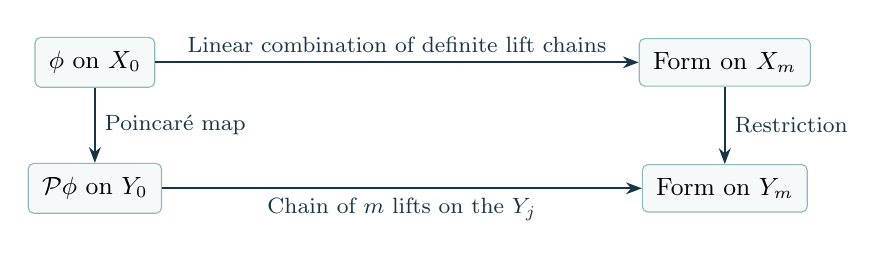
\begin{tikzpicture}[x=1cm,y=1cm,>=Stealth,
  obj/.style={draw=ocean!48,rounded corners=2pt,fill=ocean!4,inner sep=5pt,font=\small},
  lab/.style={font=\footnotesize,align=center,text=ink}]
  \node[obj] (a) at (0,1.35) {\(\phi\) on \(X_0\)};
  \node[obj] (b) at (8.0,1.35) {Form on \(X_m\)};
  \node[obj] (c) at (0,-.25) {\(\mathcal P\phi\) on \(Y_0\)};
  \node[obj] (d) at (8.0,-.25) {Form on \(Y_m\)};
  \draw[->,semithick,ink] (a)--node[lab,above]{Linear combination of definite lift chains} (b);
  \draw[->,semithick,ink] (c)--node[lab,below]{Chain of \(m\) lifts on the \(Y_j\)} (d);
  \draw[->,semithick,ink] (a)--node[lab,right]{Poincaré map} (c);
  \draw[->,semithick,ink] (b)--node[lab,right]{Restriction} (d);
\end{tikzpicture}
\end{center}

For \(j<m\) the difference in ranks is \(\dim Y_j-\dim X_j=m-1-j\). The extra block consists of hyperbolic pairs and, in odd length, a middle line. At step \(m-1\) the ranks meet. At the final step \(Y_m\) is a definite codimension-one subspace of \(X_m\). This reversal accounts for the restriction and its normalization at \(N\).

For fixed real evaluation data there is one nonzero scalar \(c_{\rm ss}\) such that for every twist \(\xi\) there are chain data \(\Psi_\xi\) for which
\begin{equation}\label{eq:bridge-seesaw}
   \Theta^{\rm raw}_\xi(\mathcal P\phi)=
          c_{\rm ss}\,B_{\xi,\Psi_\xi}\phi
       \qquad (\phi\in S_{\rm ram}).
\end{equation}
Pair the left side with any final test form. Unfolding the Poincar\'e series gives an integral against the character of the Bessel subgroup, called a Bessel period. At a single step the theta kernel transfers this period and shortens the extra block. Each transfer contributes a real integral and a finite sum of classes. After the last transfer the pairing is exactly the pairing with a restricted definite lift. The reciprocals of stabilizer indices in the finite sums introduce denominators only above the conductor of the twist. This supplies the required integrality of the coefficients away from that conductor. For the trivial twist the sum of their complex sizes is bounded as well. The scalar in \eqref{eq:bridge-seesaw} is common to all twists and all vectors. The coefficient family can depend on the twist. The rank of the resulting images will be obtained from a separate calculation. \src{src/New/UpperBound/Seesaw/SeesawIdentity.lean}{the iterated seesaw identity}.

\subsection{Recovering the requested powers on a large submodule}

The requested gain across the chain is
\[
 g_p=m\left(\sum_{\tau\in\Phi_a}s_p(a,\tau)+
              k\sum_{\tau\in\Phi}s_p(\kappa(\tau),\tau)\right).
\]
The first sum records long rows, the second the ordinary directions whose cost must also be recovered in the lower bound. A collision occurs when a long row at \(\tau\in\Phi_a\) has another long row at \(-p^e\tau\in\Phi_a\). The partner can consume the gain of the first row. Charging \(a/p^e\) for every such collision at every step gives the correct valuation up to an acceptable error at the nonexceptional nonsplit primes. At some inert primes a small \(e\) repeats the loss \(m\) times. In the source the exceptional condition is \(p\not\equiv\pm1\pmod m\) and \(\operatorname{ord}_{Q}(-p)\) odd and at most \(\lceil\log_p m\rceil\), in addition to inertness. The gain vanishes outside nonsplit primes below \(x_1\).

Fix a \(p\)-adic embedding above one such exceptional prime. From each pair of conjugate finite primes induced by \(\Phi_a\) choose one member. Every colliding pair meets this choice. The normalized Hecke operator attached to each marked prime is a sum of lattice-neighbor correspondences, multiplied by a power of \(p\) fixed by its long rows. Moving the product \(U\) of these operators through the chain carries the extra powers to the marked coordinates. The jet estimate with the corresponding long rows removed now achieves the required exponent up to a controlled loss. In particular, on \(U^m L_p\), with \(L_p\) the integral source module, the raw lift has valuation at least \(g_p-2L(p)\), where
\[
 L(p)=\frac{fa(\log b)^2}{p}
          \begin{cases} m,&p\equiv\pm1\pmod m,\\
                         1,&\text{otherwise}.\end{cases}
\]
On \(p^{j_p}L_p\) with \(j_p=\lceil 2mfa/p\rceil\) the same inequality follows by the crude collision count. The sum \(U^mL_p+p^{j_p}L_p\) thus has high valuation and contains substantially more vectors than those forced by the scalar \(p^{j_p}\) alone. \src{src/New/UpperBound/Divisibility/LocalDivisibility.lean}{marked primes and divisibility of the composite}.

The remaining issue is its index. In the model of diagonal elementary divisors \(p^{t_i}\) over \(\mathbb Z_p\), the index exponent in a sum of this form is \(\sum_i\min(t_i,j_p)\). For the actual valuation ring, which need not be discrete, the theorem bounds determinants of change-of-generators matrices. To obtain the bound, factor the Hecke correspondence through functions on neighboring lattice pairs. Intermediate edge congruences admit a near inverse to the map which sums functions over the edges. Their restrictions leave only a bounded number of additional generators modulo the chosen precision. Nakayama's lemma converts this generator bound into control of the image. The two endpoint lattices have controlled colengths as well. Adding these costs gives a bound \(L(p)h\) in powers of \(p\) for the exceptional-prime module above. This is a bound on the total loss for a family of vectors, even if particular elementary divisors have high valuation. \src{src/New/UpperBound/ElementaryDivisors/ElementaryDivisorTheorem.lean}{elementary divisors of the edge operator}.

At \(p=N\), where the upper description has gluing denominators, the cost is treated separately. In elementary terms, homogeneous monomials of degree \(a\) in \(k\) variables have mean degree \(a/k\) in each coordinate by symmetry. For diagonal rescaling by \(N\) in that coordinate, the colength is the sum of the degrees over the monomials. The corresponding mean-degree bound on the relevant weight coordinates controls the changes of local lattices under the \(m/2\) powers of the level operator. The formal bound allows the exponent \(2mfb\) for the local loss. On summing this term and the losses at small nonsplit primes one obtains nonnegative \(e_p\) with \(\sum_p e_p\log p\le \mathcal E:=fa(\log b)^3\). At each embedding there is a submodule of integral ramified source forms of colength dividing \(p^j\), \(j\le e_p h\), on which \(B_{\xi,\Psi}\) has valuation at least \(g_p-e_p\). One submodule works for every twist of conductor prime to \(p\) and every permitted chain datum. \src{src/New/UpperBound/Divisibility/ColengthAtLevel.lean}{mean degree at the level prime}, \src{src/New/UpperBound/Divisibility/LocalDivisibility.lean}{simultaneous local bounds}.

\subsection{The complex size, the level, and the index}

Put
\[
 c_B=\prod_{p\text{ small nonsplit or }p=N}p^{-\lfloor g_p-e_p\rfloor},
 \qquad \mathcal P_s=c_B c_{\rm ss}^{-1}|G|\,e_0s\mathcal P
                      \big|_{S_{\rm ram}}\quad (s\in G).
\]
The floor ensures that multiplying by \(c_B\) preserves the required local integrality on the submodules just constructed. Its finite support has \(\sum\log p\le b\), so
\[
            \log c_B\le -\sum_p g_p\log p+\mathcal E+b.
\]
Multiplication by this positive rational rescales every conjugate complex squared norm by the same factor \(c_B^2\). The multiplier \(|G|\) clears the finite-group projector. This explains the different roles of divisibility and colength. Divisibility can be spent on the common complex size, whereas the price of having restricted the source is still payable separately at the finite places.

The charge for a complex derivative of order \(j\) is
\[
        s_\infty(j)=\log(j!)+j\log(M/\Omega).
\]
Set \(H_{\rm dir}=\sum_{\tau\in\Phi}(s_\infty(\kappa(\tau))-s_{\rm fin}(\kappa(\tau),\tau))\) and \(H=mkH_{\rm dir}\). The fixed-modulus calculation in Section~\ref{sec:observable} and the CM area formula in Section~\ref{sec:setup} supply the same constant \(c_1\). The simultaneous period normalization uses a unit at every finite place. A separate scalar normalizes the vacuum so that its values are integral. In the period calculation the absolute different of \(E\) has generator equal to a unit phase times the relative-different generator times \(\sqrt{-d}\). For \(C=M\mathrm{rd}_E/(2\pi)\), the relation \(\log(M/\Omega)=1+c_1+\log C\) now gives the bound with the precision required for \emph{each} conjugate:
\[
       s_\infty(a)-s_{\rm main}\le
                  a\log(\bar\kappa C)+1+\tfrac12\log a .
\]
Indeed the \(+a\) cancels the linear term in Stirling's bound, and \(ac_1\) is removed by the expected finite gain. \src{src/Lib/CM/ChowlaSelberg.lean}{simultaneous period normalization}, \src{src/New/Derivatives/Field/PrimeDecomposition.lean}{the absolute different}, \src{src/New/UpperBound/Size/ArchimedeanSize.lean}{the one-row estimate}.

At the reversal of the towers, restriction has a scalar formed from powers of the conjugates of \(\bar\pi_N\), with \(\pi_N\bar\pi_N=N\). Its squared size is \(N^{-\sum n_\tau}\), and the endpoint weight computation gives \(\sum n_\tau=N_a a-fm\Delta/2\). Thus \(-N_a a\log N\) enters once at the last restriction. The level window \eqref{eq:Nlevel} gives \(m\log(\bar\kappa C)-\log N\le\log C+(15/2)\log b\), an error with no factor of \(m\). With the Stirling error and the scale bounds, one gets
\[
          m(s_\infty(a)-s_{\rm main})-a\log N\le32a\log b.
\]
At each step the short ordinary rows still contribute their common main amount. By \eqref{eq:bridge-finsum},
\[
     2\sum_p g_p\log p =
      m\sum_{\tau\in\Phi_a}s_{\rm fin}(a,\tau)
      +mk\sum_{\tau\in\Phi}s_{\rm fin}(\kappa(\tau),\tau).
\]
Subtracting these finite gains leaves \(H-m\mathcal R\) up to the bounded errors. The two terms have different origins. The first comes from all the ordinary rows, the second from the signed excess of the long rows. \src{src/New/UpperBound/Divisibility/ChainValuation.lean}{the last restriction}, \src{src/New/UpperBound/Size/ArchimedeanSize.lean}{the chain-size estimate}.

\paragraph{Theorem A.} Put \(L=fa(\log b)^4\). The source \(S_{\rm ram}\) is spanned by globally integral \(\phi\) for which, simultaneously for every \(s\in G\) and every complex field automorphism \(\sigma\),
\begin{equation}\label{eq:bridge-short}
              \|\Theta_1(\mathcal P_s\phi)\|_\sigma^2
                        \le \exp(H-m\mathcal R+L).
\end{equation}
For a finite set \(J\subset G\), any finite family of target vectors drawn from images \(\mathcal P_s\) of integral ramified vectors with \(s\in J\) has index at most \(2|J|h'\mathcal E\). Precisely, for each identification \(\iota:\mathbb C\simeq\overline{\mathbb Q}_p\), an integral matrix of combinations makes every member's lifts integral for all admissible \(m\)-fold twists of conductor prime to \(p\); an \(m\)-fold twist stays ramified at every conductor place in its first \(m\) powers. The weighted sum of the permitted determinant valuations is bounded by the stated index. Group the vectors by the translate used and add the local colength bounds on the blocks. The inequality \(h\le2h'\) gives the factor two. For the size bound, the cost of the initial short forms, the norm of the good projection and the rounding costs in \(c_B\) together fit in \(L\). The quantifiers on the two conclusions differ in a necessary way. Archimedean shortness uses the untwisted lift at all complex conjugates. Finite-place integrality must hold for a whole family of twists at once. \src{src/New/Reduction/ShortAndEnough.lean}{the two assertions of Theorem A}.

\section{Theorem B. How many short images are independent?}\label{sec:bridge-enough}

The size bound for a family of vectors is compatible with every vector lying on one line, even with every vector being zero. What rules that out here is a pair of moment calculations. One keeps track of the norm surviving the projection to the target. The other measures how much of the same norm can keep appearing in overlapping translates. The normalization coefficients of their automorphic inputs are essential because a fixed multiplicative error in the second moment could leave a fixed fraction of all the target dimensions unaccounted for.

\subsection{The finite projector and a common mass}

The group \(G\) acting at the chosen places above \(p_0,p_1\) is a product of finite general linear groups of rank \(r\). At a place with residue field \(\mathbb F_q\), a monic squarefree polynomial of degree \(r\) with nonzero constant term labels a Green character and hence a central projector. The good projector \(e_0\) sums the tensor projectors for the families of labels satisfying both of the following tests. At every chosen place the polynomial has no root in \(\mathbb F_q\) of order dividing \(q_2\). Above each of \(p_0,p_1\), at least one polynomial has as a root a generator of \(\mathbb F_{q^r}^\times\). This last polynomial is irreducible. Its local test function is cuspidal, meaning that its integrals along the unipotent radicals of proper parabolics vanish. It supplies a place for a trace comparison. The root exclusion has a different purpose: a weighted average over the subgroup fixing a specified hyperplane acts as zero on the retained types whenever its character parameter is a forbidden root. This vanishing will also be used for the periods of false lifts. Requiring a primitive place above both level primes permits the subsequent Galois argument to choose a witness away from a given coefficient prime.

The price of the tests can be computed in the regular representation. For \(A=\sum_g a_g g\), the trace of left multiplication is \(|G|a_1\). Thus the identity coefficient of a projector gives its relative rank, and a label of degree \(d_\lambda\) has mass \(d_\lambda^2/|G|\). In each residue field a prescribed forbidden linear factor leaves at most \(q^{r-1}\) monic polynomials; a union over possible repeated factors gives another loss bounded by \(rq^{r-1}\). Meanwhile \(\varphi(q^r-1)/r\) labels are primitive, by counting generators in Frobenius orbits. The lower bound \((1-r/q)q^{-r}\) for the mass of a label turns these counts into a bound for tuples of labels. The cost of one forbidden label is estimated by summing over places, while the chance of missing a primitive label in all \(f\) factors has an exponentially decaying upper bound. At each of the two level primes the identity coefficient of the discarded projector is at most \(1/(2b^8)\). The automorphic moment calculation is still needed to transfer a regular-representation count to the actual forms. \src{src/New/UpperBound/Objects/LabelsAndIndexTypes.lean}{polynomial labels and good families}, \src{src/New/Spanning/MainTerm/BadTypes.lean}{weighted count of the excluded types}.

Let \(d_T=\dim V\). Matching traces of spherical Hecke operators on these good subspaces compares multiplicities on \(Y_0\) with those on a definite rank-\(r\) space. The comparison is made for each selected type and added over the good types. On the definite side the free principal level gives a dimension bound by class counting. If \(D_\infty\) is the product of the Bessel formal degrees at infinity and \(\mu_r\) is the mass of the genus of the standard rank-\(r\) lattice, the bound reads
\[
                      d_T\le |G|D_\infty\mu_r .
\]
Here the mass is the sum of the inverse orders of lattice automorphism groups. Exactly the same product \(D_\infty\mu_r\) occurs in the denominator in the second moment. The match is why a dimension estimate involving these particular local types is required. \src{src/New/Spanning/Multiplicities/EqualMultiplicities.lean}{comparison of Hecke multiplicities}, \src{src/New/Spanning/SecondMoment/SpanningTheorem.lean}{the target dimension}.

\subsection{The two moment estimates}

For this calculation let \(P\) be the normalized Poincar\'e map on the full source of dimension \(h\), taking values in the entire principal-level space. Its scalar normalization is determined by the Haar volume and the covolume of the unipotent quotient. The scalar and coordinates differ from those used for \(\mathcal P_s\); the ranges after projection and restriction agree up to nonzero scalar. For any source subspace \(U\), let \(\pi_U\) denote orthogonal projection. The two estimates are
\begin{align}
 \|e_0 P\pi_U\|_{\rm HS}^2&\ge \dim U-5b^{-4}h,\label{eq:bridge-isom}\\
 \frac{d_T}{|G|}\sum_{s\in G}\|P^*sP\|_{\rm HS}^2
                 &\le (1+9b^{-4})h^2.\label{eq:bridge-moment}
\end{align}
The Hilbert--Schmidt norm squared is the sum of the squared absolute values of matrix entries in orthonormal bases.

One can see exactly which matrix entries are being counted. Label a source coordinate by a definite lattice class \(c\) and an index \(i\) of the Bessel function at infinity. In the block \((c,s,c')\), unfolding gives a sum of matrices indexed by rational \(\gamma\) for which \(h_c^{-1}\gamma h_{c'}\) is integral and reduces to \(s\). An entry is an integral pairing two Bessel components at \(y\) and \(\gamma^{-1}y\) against the class cutoffs. The block is obtained with the factor \(1/\nu\) for the unipotent covolume (and conjugation according to the matrix-entry convention). Its squared Frobenius norm therefore sums over pairs \(\gamma,\gamma'\) in the same block.

At the identity, the contributions in the Bessel subgroup give the identity operator. The squared error is \(\|P^*P-I\|_{\rm HS}^2\le b^{-12}h\). Controlling the same pairings after applying the two complementary type projectors bounds the portion discarded by \(e_0\), which proves \eqref{eq:bridge-isom} for every \(U\). For the full-group average, the infinite-place test functions can be cut off with very small tail error because the discrete-series weights have a large gap. Integral bounds for the cut Bessel kernels control each orbit. Squaring the class sums leads to two different arithmetic counts.
\begin{itemize}
 \item Two rational elements in one block give lattice frames congruent at the level. For frames with different link subspaces, or with a degenerate discriminant, the common lattice and its discriminant supply a saving. Congruence at the primes of \(M\) forces a divisibility of discriminants. Bounding the number of lattices of a given corank and using a weighted Schur estimate makes the combined contribution of these terms at most \(b^{-kf}\) times the identity second moment.
 \item For pairs with the same link in the open cell, unfolding gives local orbital integrals. At finite places these give generalized Kloosterman sums. The real and finite positive kernel estimates combine into a global sieve via Poisson summation. Fixing a nonzero frame vector at each of \(j\) selected places saves a factor \(b^{-6kj}\) in the normalized main term. On the other reductions one controls the failure of a leading minor to be nonzero by finite-field averaging. Together with the degenerate-pair bounds and the terms on the scalar cosets, this yields
 \[
       \sum_{s\in G}\|P^*sP\|_{\rm HS}^2
          \le (1+9b^{-4})\frac{h^2}{D_\infty\mu_r}.
 \]
\end{itemize}
Multiplying by the dimension bound gives \eqref{eq:bridge-moment}. The coefficient approaching one, and the independence from the unknown mass, both matter to the application. \src{src/New/Spanning/Unfolding/Moments.lean}{the operator and amplitude identities}, \src{src/New/Spanning/RemainingTerms/Sum.lean}{pairs of lattice frames}, \src{src/New/Spanning/MainTerm/EnergyEstimate.lean}{the open-cell sieve}, \src{src/New/Spanning/Unfolding/MomentBounds.lean}{the whole-group estimate}.

\subsection{Restriction followed by greedy selection}

There is a short argument from these two estimates to rank. Put \(\eta=1/(8b^2)\), which bounds both \(5b^{-4}\) and \(9b^{-4}\). Inside the target let \(F\) have dimension \(\alpha d_T\), and set \(K_G=|G|^{-1}\sum_{s\in G}sPP^*s^{-1}\). Cyclicity of trace gives \(\operatorname{tr}(K_G^2)=|G|^{-1}\sum_s\|P^*sP\|_{\rm HS}^2\). Thus Cauchy--Schwarz for the matrices \(\pi_F,K_G\) shows that the average of \(\|\pi_F sP\|_{\rm HS}^2\) is at most \(h\sqrt{\alpha(1+\eta)}\). Choose an \(s\) at or below this average. On the inverse image of \(F\) under \(e_0sP\), the maps \(e_0sP\) and \(\pi_FsP\) agree. Since \(e_0\) commutes with translation and the action is unitary, \eqref{eq:bridge-isom} applies to the first map on that subspace. Using \(\sqrt{\alpha(1+\eta)}\le (1+\alpha+\eta)/2\), we obtain
\[
   \dim (e_0sP)^{-1}F
     \le \bigl((1+\alpha)/2+3\eta/2\bigr)h.
\]
For every current span \(F\) one translate has a preimage this small. That is the spreading property used in the source.

In the implementation on the cited revision one first restricts this property to \(S_{\rm ram}\), then chooses the translates. Here are the constants which make the order work. We have \(h'\ge(1-\eta)h\) and the scales imply
\[
     (1+3\eta/2)h\le(1+3\eta)h'.
\]
Write \(a_F=(1+\alpha)/2\le1\). Since
\((a_F+3\eta/2)h-(a_F+3\eta)h'\) is increasing in \(a_F\), the same inequality with \(a_F\) in place of \(1\) follows. The inverse image inside \(S_{\rm ram}\) is contained in the full inverse image, so the additive loss in the spreading estimate on the smaller source is \(3\eta\). In the greedy lemma this is \(3\eta'/2\) with \(\eta'=2\eta\). All subsequent images are images of the required ramified source.

If a fraction \(1-\alpha>16(2\eta)\) of the target remains missing, adjoining the chosen image increases rank by at least
\[
   \bigl((1-\alpha)/2-3\eta\bigr)h'
            \ \ge\ \tfrac25(1-\alpha)h'.
\]
The uncovered dimension contracts by a factor at most \(1-2h'/(5d_T)\). Iteration down to the stated threshold requires a number of translates bounded by a logarithm times \(d_T/h'\). Nontriviality of the full source and \eqref{eq:bridge-isom} give \(d_T>0\). Thus \textbf{Theorem B} supplies a set \(J\subset G\) such that
\begin{equation}\label{eq:bridge-enough}
  |J|h'\le5d_T\log(1+2b^2),\qquad
  \dim\sum_{s\in J}\mathcal P_s S_{\rm ram}
                         \ge(1-4/b^2)d_T .
\end{equation}
The same \(J\) now gives independent vectors from Theorem A and bounds their index. The order of restriction accounts for the deficit \(4/b^2=16(2\eta)\). \src{src/New/Spanning/SecondMoment/FewTranslates.lean}{restriction of spreading and greedy covering}, \src{src/New/Reduction/ShortAndEnough.lean}{Theorem B on the ramified source}.

\section{Theorem C. The lower bound for the volume of theta lifts}
\label{sec:arithmetic-lower}
Continue to write $V$ for the space of good target forms on $Y_0$, with $d_T=\dim_{\mathbb C}V$.
The parameter $d$ specifying the imaginary quadratic field remains fixed throughout this construction.
For a twist $\xi$, let $\Theta_\xi$ denote the chain from $V$ to forms on $Y_m$. Write
\[
 Z(\xi)=\det(\Theta_\xi^*\Theta_\xi),\qquad
 H_{\rm dir}=\sum_\tau\bigl(s_\infty(\kappa_\tau)-
                      s_{\rm fin}(\kappa_\tau,\tau)\bigr),
 \qquad H=mkH_{\rm dir}.
\]
The quantity $H_{\rm dir}$ records the cost at infinity of the derivatives in one ordinary direction, less their forced prime divisibility. The upper bound paid for $k$ such directions at each of $m$ lifts. We will recover this whole amount as a lower bound. Precisely, suppose independent $y_1,\ldots,y_n\in V$ satisfy the index bound $\delta$ and the logarithmic squared-covolume bound $c$ for the target twisted lattice. Then Theorem C asserts
\begin{equation}
 n\ge (1-4/b^2)d_T\quad\Longrightarrow\quad
 c+2\delta\ \ge\ d_T\bigl(H-3fa(\log b)^4\bigr).
 \label{eq:lowlong}
\end{equation}
There are three mathematical issues here. We need a formula for the volume change through an entire chain. We must estimate its finite-place denominators without restricting which Dirichlet character occurs in the final theorem. Finally, since the volume change is defined in dimension $d_T$, we must complete the given vectors to a basis. We take these in turn.
\sources{\src{src/New/Determinant/Twist/LongForms.lean}{Statement and proof of Theorem C}.}

\subsection{Exchanging two theta integrals}
On the arrow $Y_i\to Y_{i+1}$ the ranks are $r+it$ and $r+(i+1)t$.
The available Rallis inner-product formula requires twice the source rank to be less than the target rank. This is true for $i=0$, since $t=5r$, and fails for $i\ge1$. There is a second issue familiar from linear algebra. Given maps $A$ and $B$, the Gram operator of $BA$ is $A^*(B^*B)A$. To compute its determinant one must know how the Gram form of $B$ restricts to the image of $A$.

The elementary move that overcomes both difficulties compares theta integrals from two complementary spaces $V,V'$ to a common space $W$. In the exchange theorem their ranks satisfy
\[
 \dim W=\dim V+\dim V',\qquad \dim V=\dim V'+2e .
\]
The signatures match, and with $q_-$ negative signs on $W$ the inequalities $2q_-+2\le\dim W\le2\mu_\tau+2q_-$ hold at each infinite place for the specified weight $\mu_\tau$. Fix an archimedean Schwartz vector on the smaller side. The theorem supplies a partner on the larger side, chosen before the modulus and tame character. With compatible splitting characters and matched finite test functions, integration over $[U(V)]$ gives $c_\nu$ times integration over $[U(V')]$, as functions on $U(W)$. The magnitude is
\[
 |c_\nu|^2=C\prod_{w\in S} q_w^{e^2}
                  \prod_{z=1}^{e}|L^S(z,\nu)|^2>0 .
\]
Here $C>0$ belongs to the fixed data, $S$ consists of the modulus places, and a superscript $S$ on the partial Hecke function uses the source's convention of omitting $S$ and its conjugate. The theorem allows $c_\nu$ to depend on the character and modulus. The proof unfolds the theta kernel for a split isotropic frame, factors the kernel on an orthogonal sum, and compares complementary integrals on matched data. Equal-rank theta periods supply the normalization. Locally, a common system of symmetric representatives for lattice cosets lets the same finite section be read from either system of matrix coordinates.
\sources{\src{src/New/Determinant/Exchange/LargeTriple.lean}{Parabolic terms and equal-rank periods},
\src{src/New/Determinant/Exchange/MatchingPartners.lean}{Matching finite sections},
\src{src/New/Determinant/Exchange/TheoremForPartners.lean}{Complementary-space exchange}.}

Apply this identity on a direct sum of two spaces. A product of two kernels may be read as a lift followed by a transposed lift. Changing the intermediate space gives the two routes round a square. At this point the asserted relation is between the appropriate sums over matched finite data. Its factor takes the form $\kappa/c_\nu$ with $\kappa$ independent of the twist. The square theorem alone allows $\kappa=0$.
\sources{\src{src/New/Determinant/Exchange/OneSquare.lean}{The two routes round one square}.}

Arrange the lifts by the interval of blocks present. Adding the next block on the right extends an interval. A descent removes the leftmost block. Sliding a descent across the additions moves it to the beginning of the interval, where a single lift and descent can be evaluated. For example, in a row of three blocks the first descent crosses blocks $2,3$ and the second descent crosses block $3$. Those moves produce the pairs $(1,2),(1,3),(2,3)$. Since the twist on block $j$ is $\xi^j$, crossing blocks $i,j$ leaves a quotient character twisted by $\xi^{j-i}$. In the current realization one induction on interval length carries both commutation and inner-product identities needed at a move. It tracks the scalar for moving the descent past the row at the same time as the scalar in the inner product. Level factors are computed by counting block upper triangular invertible matrices. The inductive zero-vector test starts with an empty interval. It commutes a descent along a row that kills a vector, then uses injectivity at the rank-$r$ stem of the shorter row. Thus the chain is injective and its Gram determinant is positive. This permits division in the assembled determinant formula.
\sources{\src{src/New/Determinant/Chain/TriangleNorms.lean}{The joint induction for chain identities},
\src{src/New/Determinant/Chain/ChainNorms.lean}{Weighted chains and their level factors}.}

For each $j$ there is now a single lift $u_{j,\eta}$ from the good forms on $W_j$ of rank $r$ to forms on a definite space of rank $r+t$, with $\eta=\xi^j$. It lies in the stated convergence range. In the doubling argument the two arguments of the inner product are put on $W_j\oplus W_j^-$, with the form negated in the second summand. In the Siegel--Weil formula the support of the test datum removes every contributing maximal isotropic space except graphs of rational isometries. Summing over those isometries unfolds one quotient integral. What remains is a convolution operator given by the Rallis series. Its determinant is initially computed on good forms on $W_j$. Equality of multiplicities for Hecke systems on $W_j$ and $Y_0$ moves it to the common $d_T$-dimensional space $V$. In the finite-dimensional trace comparison this also follows by matching the traces of powers, which determine the characteristic polynomial.
\sources{\src{src/Lib/SiegelWeil/RallisInner/Doubling.lean}{Doubling in the convergence range},
\src{src/New/Spanning/Multiplicities/EqualMultiplicities.lean}{Comparing the Hecke spectra}.}

Write $R_j$ for the resulting operator on $V$, $q(\xi)=\prod_{w\in Q(\xi)}q_w$, and $Z_j(\eta)=\det(u_{j,\eta}^*u_{j,\eta})$. There are constants $A_j\ne0$ independent of $\xi$ and a common modulus factor $c_{\rm lev}$ such that
\[
 \Theta_\xi^*\Theta_\xi=c(\xi)c_{\rm lev}^m\prod_{j=1}^m R_j,
 \qquad Z_j(\xi^j)=(A_jc_{\rm lev})^{d_T}\det R_j .
\]
The common $c_{\rm lev}$ exists because the first $m$ powers ramify on the same support. Taking the determinant of the first equality and substituting the second cancels $c_{\rm lev}^{md_T}$. Dividing by the resulting formula for the trivial twist and using the positive Gram determinants gives
\begin{align}
 \frac{Z(1)}{Z(\xi)}
 &= S(\xi)^{-d_T}\prod_{j=1}^{m}\frac{Z_j(1)}{Z_j(\xi^j)},&
 S(\xi)&=q(\xi)^{e_0/2}\prod_{1\le i<j\le m} R_{ij}(\xi).
 \label{eq:arithchain}
\end{align}
The exponent $e_0\in\mathbb Z$ is fixed. Each $R_{ij}$ is a product of $t$ partial Hecke-value ratios of the quotient of the lift characters at the power $j-i$. The exponent $d_T$ is the dimension on which the scalar acts. In this notation $Z_j$ takes a single character. The Lean declaration takes an $m$-fold character and the index $j$, and forms its $j$th power internally.
\sources{\src{src/New/Determinant/Chain/NormOfChain.lean}{Positivity and chain factorization}.}

\subsection{A comparison operator for a single lift}
Fix $j$ and suppress it in the notation. Put $u=u_{j,\eta}$, $Z=\operatorname{im}u$, and let $P_Z$ be orthogonal projection. For an endomorphism $U$ of the ambient space there is a determinant identity
\[
 \det(u^*u)\det(P_ZU|_Z)=\det(u^*Uu).
\]
Indeed $u$ gives an isomorphism from its source onto $Z$, and $u^*$ kills $Z^\perp$. Composing $u^*u$ with the pullback of $P_ZU|_Z$ along this isomorphism gives $u^*Uu$. The choice of $U$ determines whether either side can be estimated.

Let $g_\eta$ glue a tuple of forms on a smaller definite unitary group into a form on the target of $u$. Its adjoint measures periods on that subgroup. Three exchanges compare the period map for different twists. They yield a nonzero scalar $c'_\eta$ for which $c'_\eta g_\eta^*u_{j,\eta}$ is a single fixed map $u^\circ$. A period nonvanishing argument gives this fixed map zero kernel. Moreover $|c'_1|^2/|c'_\eta|^2=P_j(\eta)/P_j(1)$, where $P_j$ is an explicit product of squared absolute Hecke values and local factors. Set
\[
 U_\eta=n_{\rm Aut}\,h_j^2\,g_\eta g_\eta^*,\qquad
 \Delta_\eta=\det(P_ZU_\eta|_Z),\qquad \rho_\eta=P_j(\eta)/P_j(1).
\]
The multiplier $n_{\rm Aut}$ clears stabilizer orders in class sums, and $h_j$ is the hook product of a weight diagram. The preceding identity for adjoints gives $u^*U_\eta u=n_{\rm Aut}h_j^2|c'_\eta|^{-2}(u^\circ)^*u^\circ$.
The positivity of the fixed Gram form justifies cancelling its determinant and yields
\begin{equation}
 \frac{Z_j(1)}{Z_j(\eta)}
       =\frac{\Delta_\eta}{\Delta_1}\,\rho_\eta^{-d_T}.
 \label{eq:arithcomp}
\end{equation}
\sources{\src{src/New/OneLift/ComparisonOperator/ThreeExchanges.lean}{The three exchanges},
\src{src/New/OneLift/ComparisonOperator/GluingMaps.lean}{Gluing and period maps},
\src{src/New/OneLift/LiftVolumeHeight.lean}{Compression determinant identity}.}

The operator has two further properties that make \eqref{eq:arithcomp} arithmetic. An integral tight frame for the tuple space writes $U_\eta$ as a sum of rank-one operators with controlled coefficients. It takes integral forms to integral forms at every prime away from $Q(\eta)$. Also $U_\eta z$ is orthogonal to false lifts for every $z\in Z$. At a split place off the level a false lift has the good local type, belongs to $Z^\perp$, and is killed by the Hecke polynomial at the prescribed lift root. Vanishing of its first descent and of certain sums over hyperplanes gives vanishing up a tower obtained by adjoining hyperbolic planes. Reading a Fourier coefficient at the top gives zero for the block periods that enter the gluing. This supplies the precise orthogonality needed after applying $U_\eta$ to a genuine lift.
\sources{\src{src/New/OneLift/FalseLifts/PeriodsOfFalseLifts.lean}{Period vanishing up the tower},
\src{src/New/OneLift/LiftVolumeHeight.lean}{Integrality and orthogonality of the comparison operator}.}

Write $h((y_\iota))\le C$ for the source's height bound. The family is indexed by a prime $\ell$ and a field isomorphism $\iota:\mathbb C\simeq\overline{\mathbb Q}_\ell$. One multiplier $H_0\ne0$ has all complex conjugates at most $e^\alpha$, while $|\iota(H_0 y_\iota)|_\ell\le\ell^{h_\ell}$ with $h_\ell\ge0$, and $\alpha+\sum_{\ell\in F}h_\ell\log\ell\le C$ for every finite set $F$ of primes. Products add the bounds. A varying family can have negative height bound. For example choose $y_\iota=9$ at $\ell=3$ and $y_\iota=1$ elsewhere. Taking $H_0=1/9$ gives zero finite cost and $\alpha=-\log9$. For the constant family $1$, boundedness at every identification over $2$ forces its multiplier to be algebraic. Taking its field norm to $\mathbb Q$ and applying the rational product formula gives $C\ge0$. This distinction explains why local choices of $\xi_\iota$ can eventually give a positive lower bound on a fixed complex volume.
\sources{\src{src/New/Reduction/Lattices/Heights.lean}{Multipliers and the product formula}.}

Choose a regular family of twists, whose existence is proved below. Its denominator allowance for each $j$ consists of logarithmic costs $\beta_\ell$ with
\[
 \sum_{\ell\in F}\beta_\ell\le B_{\rm den},
 \qquad B_{\rm den}=\frac{fa(\log b)^3}{mk}.
\]
At $\iota$ and $\eta=\xi_\iota^j$, some operator $\Lambda$ on $Z$ clears $P_Z$ on integral forms orthogonal to the false lifts and satisfies $|\iota(\det\Lambda)|_\ell\ge e^{-d_T r\beta_\ell}$. Thus $\Lambda P_ZU_\eta|_Z$ preserves integral lifts. Scale an eigenvector to have maximal integral gauge equal to one. Its image then shows that the eigenvalue has norm at most one. Multiplication of eigenvalues bounds $|\iota(\Delta_\eta)|_\ell\le e^{d_T r\beta_\ell}$. At infinity the untwisted operator bound gives $|\sigma\Delta_1|\le e^{3d_T fmb(\log b)^2}$ for every conjugate. The common multiplier $\Delta_1$ therefore controls the first factor of \eqref{eq:arithcomp}. The term of size $-kH_{\rm dir}$ in the one-stage bound comes from the special values in the other factor.

\subsection{Why the critical values recover exactly $k$ directions}
For a critical pair $(\nu,z)$, let $r_{\nu,z}(\eta)$ be the ratio of the magnitudes of the partial Hecke values at $z$ for $(\nu\eta)^{-1}$ and $\nu^{-1}$. Both omit the chosen level places and their conjugates. The numerator also omits $Q(\eta)$ and its conjugate. These functions are those of characters of the CM field obtained from $U(1)$ by $x\mapsto x/\bar x$. Their critical values enter as coefficients in the proof of the zero-free theorem for Dirichlet $L$-functions.

There are three lists of critical values for a single comparison. Their endpoints are
\[
 z_*=7m/2+k/2,\qquad m,\qquad m/2.
\]
The chosen $k,m$ are even. The terms $7m/2<z\le z_*$ in the first list are \emph{main pairs}. Their tame character is fixed at the chosen places, and their weights are close to those of lift $j$. Their row lengths $l_\tau=c_\tau-z$ satisfy $\kappa_\tau\le l_\tau\le\kappa_\tau+x^{42}$. There are exactly $k/2$ of them. The other terms consist of the first $7m/2$ entries of that list and the whole of the two shorter lists, exactly $5m$ entries. All of these are ramified pairs, with a specified sign $s=1$ or $-1$. The exchange calculates \emph{squared} magnitudes. Consequently
\[
 \rho_\eta=q(\eta)^{e_j}
    \left(\prod_{p\,\mathrm{main}}r_p(\eta)
                 \prod_{p\,\mathrm{other}}r_p(\eta^{s_p})\right)^2 .
\]
The exponent $e_j$ is the sum of the squares of the three endpoints. A rational power of the positive conductor norm costs zero in the family height when its underlying prime $\ell$ does not divide that norm. The regular family gives each of the $5m$ other inverse ratios height bound $x_1$. A sharper bound for each main pair is the decisive step.
\sources{\src{src/New/Determinant/Twist/FitTwists.lean}{Main pairs and ramified pairs},
\src{src/New/OneLift/HeckeValues/TwistedValueHeights.lean}{The three lists and their cardinalities}.}

Let $\phi_\eta$ be the normalized lift associated with one such main pair. It lifts a character from rank one to a definite group of rank $2z$. Evaluation of the Rallis formula at this rank gives the identity
\begin{equation}
 r_p(\eta)^{-1}=q(\eta)^{2z-1}
                        \frac{\|\phi_1\|^2}{\|\phi_\eta\|^2}.
 \label{eq:arithrankone}
\end{equation}
For $\eta=1$ the comparison of the normalized norm with that of a pair with an empty weight row cancels an unknown archimedean constant. The empty-row algebraic part is integral. The factorials and the common CM period in the remaining expression give
\[
 h\bigl(\|\phi_1\|^2\bigr)\le B_{\rm den}-\sum_\tau s_\infty(\kappa_\tau).
\]
At finite places the reciprocal of the twisted norm has to be bounded from above. Choose test forms $v,v'$ at $\iota$ and its conjugate for the \emph{same} $\eta$, and let $P$ project onto the line of $\phi_\eta$. With inner products conjugate-linear in their first argument,
\[
 \langle Pv,Pv'\rangle=
 \frac{\langle v,\phi_\eta\rangle\langle\phi_\eta,v'\rangle}{\|\phi_\eta\|^2}.
\]
The numerator must contain nonzero pairings whose valuations do not grow too large. A universal divisibility assertion on theta derivatives alone would also be true for a zero pairing. We need to find test data that nearly attain the predicted divisibility.
\sources{\src{src/New/OneLift/HeckeValues/CharacterLiftNorm.lean}{The rank-one inner product},
\src{src/New/OneLift/HeckeValues/AlgebraicPartSize.lean}{Untwisted norm and weight rows}.}

The sharpness argument can be seen on one CM elliptic curve. Let $M_n$ be the largest $p$-adic absolute value of an $n$th derivative in the additive coordinate of any integral series in the formal parameter of the curve, evaluated at the origin. Only finitely many monomials contribute in degree $n$, so the ultrametric inequality realizes the maximum on a monomial. The integral formal addition law, expanded in two variables and differentiated, gives $M_{n+h}\le M_nM_h$. Explicit coefficients of the rescaled parameter at $N=q_p^a$, where $q_p$ is the quadratic residue-field size, give
\[
 M_N\ge p^{-(N-1)\gamma_p},\qquad
 \gamma_p=\frac{1}{p-1}-\frac1{e_p(q_p-1)}
\]
for arbitrarily large $a$, with $e_p$ the ramification index. A strict inequality $M_n<p^{-n\gamma_p}$ at even one positive $n$ would contradict these indices. Write $N=un+r$, $0\le r<n$, and bound $M_N p^{N\gamma_p}$ by $(M_np^{n\gamma_p})^u$ times the largest of the $n$ possible remainders $M_rp^{r\gamma_p}$. This tends to zero while the displayed lower bound stays positive. Hence some derivative in every degree has valuation at most $n\gamma_p$. At an inert prime $\gamma_p=p/(p^2-1)=p^{-1}+p^{-3}+p^{-5}+\cdots$, the same rate encountered in the upper bound.

Several infinite places can interact in the multivariable derivative. The proof separates nearby places using disjoint sets of variables, takes products on twelve copies and uses Fourier inversion to recover an indicator datum supported on one residue class. The output is a single nonzero scalar of bounded complex conjugates for all primes, and, separately for each $p$ and coefficient embedding, an indicator datum and a coefficient of the required degrees. After multiplication by the vacuum normalization and $\prod_\tau l_\tau!$, this coefficient has valuation at most the ordinary-direction local prime sum plus the valuation of the common scalar. An integral point test form then reads the coefficient in an actual pairing. Both tests satisfy false-lift orthogonality.
\sources{\src{src/New/Derivatives/Sharpness/OneCurve.lean}{Sharpness in every degree},
\src{src/New/Derivatives/Sharpness/BoundAttained.lean}{A coefficient at each prime},
\src{src/New/OneLift/HeckeValues/TwistedValueHeights.lean}{From coefficients to test pairings}.}

There is a precise account of the losses in \eqref{eq:arithrankone}. Write
$A_\eta=\langle v,\phi_\eta\rangle\langle\phi_\eta,v'\rangle$ and $r_{0,\eta}$ for the ratio of a second, ramified empty-row pair. After suppressing the conductor unit the four factors of $r_p(\eta)^{-1}$ are
\[
    \|\phi_1\|^2,\qquad
    \langle Pv,Pv'\rangle,\qquad
    r_{0,\eta}^{-2},\qquad r_{0,\eta}^{2}/A_\eta .
\]
The first has the bound just computed. The second costs $B_{\rm den}$ by the rank-one projection part of regularity. The third costs $2x_1$. The sharp coefficient, used also at the conjugate embedding, bounds the fourth by $2B_{\rm den}+\sum_\tau s_{\rm fin}(\kappa_\tau,\tau)$. Since $x_1\le B_{\rm den}$, addition gives $h(r_p^{-1})\le6B_{\rm den}-H_{\rm dir}$. Applying this to the $k/2$ main factors and taking the square gives
\[
 h(\rho^{-1})\le k(6B_{\rm den}-H_{\rm dir})+10m x_1 .
\]
The factor $k$ is now accounted for by an exact cardinality and an exact exponent. Substitution in \eqref{eq:arithcomp} and the scale bound
\[
 3fmb(\log b)^2+(r+6k)B_{\rm den}+10m x_1
      \le k(\log b)B_{\rm den}
\]
give the required bound for a single stage,
\begin{equation}
 h\!\left(\left(\frac{Z_j(1)}{Z_j(\xi_\iota^j)}\right)_\iota\right)
 \le d_T\left(\frac{fa(\log b)^4}{m}-kH_{\rm dir}\right).
 \label{eq:arithonestage}
\end{equation}
\sources{\src{src/New/OneLift/HeckeValues/TwistedValueHeights.lean}{Four-factor height estimate},
\src{src/New/OneLift/LiftVolumeHeight.lean}{The one-stage bound}.}

\section{Congruences, simultaneous twists and completion of the basis}
\label{sec:arithcong}
At a finite prime orthogonal projection can produce a denominator even for an integral symmetric operator. For example
\[
 A=\begin{pmatrix}1&3\\3&9\end{pmatrix}
\]
has eigenvectors $(1,3)$ and $(-3,1)$, with eigenvalues $10$ and $0$. Projection onto the first eigenline is $A/10$. At $2$ or $5$ the two eigenvalues become congruent, so a lattice vector can have a nonintegral projection. In the theta spaces there are many Hecke operators and many simultaneous eigensystems. The cost that enters \eqref{eq:arithcomp} is the valuation of a \emph{determinant} on the genuine lift space. Summing separate estimates for every possible pair of congruent forms would incur an uncontrolled multiplicity.

\subsection{From Hecke congruences to a controlled determinant}
Fix $\ell$ and a coefficient isomorphism $\iota$. A normalized Galois representation attached to a lift of a good eigensystem has a prescribed trace. For the rank-$r$ descent pair, with the appropriate $\ell$-adic avatar $\psi$ of the inverse twisting character, it is
\[
 \operatorname{tr} N(g)=\psi(g)\operatorname{tr} R(g)
              +\sum_{a=0}^{t-1}\chi_{\rm cyc}(g)^{-a}.
\]
Here $R$ depends on the eigensystem and index $j$ and can be fixed before the twist. The good residue labels and the weight conditions supply the needed inertia and Hodge--Tate restrictions. For sufficiently large coefficient rings the integral image of the main block spans its full matrix algebra, and a suitable inertia element acts by a scalar whose order modulo the maximal ideal is large. These are specific properties used in the cohomological calculation. The construction uses compatibility with Frobenius data in the precise form proved for the relevant Hecke systems. Its output at this interface is an equality of traces. Integral extensions still contain arithmetic information invisible to such an equality. For instance upper-triangular matrices with diagonal characters $\alpha,\nu$ and upper entry $b(g)$ have trace $\alpha(g)+\nu(g)$ for every splitting. The functions $b(g)/\nu(g)$ obey the cocycle equation for the character $\alpha/\nu$, and changing the splitting adds a coboundary. This identifies the natural objects that measure persistent congruence.
\sources{\src{src/New/Congruences/GaloisRepresentations/AttachedRepresentations.lean}{Representations of eigenforms},
\src{src/New/Congruences/GaloisRepresentations/RowsFromEigensystems.lean}{Main-summand traces},
\src{src/New/Congruences/GaloisRepresentations/SelmerHypotheses.lean}{Twisting and local hypotheses}.}

A genuine lift has $\det(1-N(g))=0$ for every $g$, by the term indexed by $a=0$ in the character string and the induced characteristic-polynomial identities. Call systems satisfying this vanishing weak lifts. There is a reason for retaining the false-lift condition in the statement about projections. A group can have eigenvalue one on every element in a representation whose global fixed space is zero. For example, let two generators of the Klein four group change respectively the signs in coordinates $(2,3)$ and $(1,3)$ of a three-dimensional space. Each nonidentity element fixes a different coordinate line. In the automorphic argument a local Hecke-string theorem and the type projection identify the weak components of the projection error, and orthogonality to false lifts removes the ones in $Z^\perp$.

For the remaining systems at base level choose, for each non-weak $y$, some $g_y$ for which $a_y=\det(1-N_y(g_y))\ne0$. Write $\delta_g(x)=\det(1-N_x(g))$. The product
\[
 D(x)=\prod_y\bigl(a_y-\delta_{g_y}(x)\bigr)
\]
vanishes on every such $y$ and equals $n_0=\prod_y a_y\ne0$ on weak systems. Dividing by $n_0$ would produce a projector of unknown cost. The proof uses this product only to separate systems at an intermediate precision.

To see which coefficient will be charged, adjoin one variable $X_v$ per ordered auxiliary prime. Relations linking tame inertia $\tau_v$ to Frobenius $F_v$ have the form
\[
       (\tau_v-1)-X_v(F_v-1)H_v(F_v),\qquad H_v(1)=1 .
\]
Traces of multiples of these relations, together with the allowed precision terms, give a module of relations in the Hecke-polynomial algebra. A first-order Ribet argument supplies one multiplier $F$ taking all the determinants $\delta_g$ into that module, and hence taking $D-n_0$ there. At the designated lift systems, every coefficient of $F$ on a proper squarefree divisor of $\prod_v X_v$ vanishes. At a selected lifted eigensystem the valuation estimate controls \(c_0^2\) times the coefficient of the full squarefree monomial, where \(c_0\) is the fixed group-order multiple used to clear stabilizers. Relations among the matrices $N(g)-1$ give relations on their cocycles. Full-sized minors present these relations by determinants. Over a discrete valuation ring their valuations measure the lengths of finite cokernels. The zeroth Fitting ideal performs this calculation simultaneously on the main block and the cyclotomic character blocks. Ordered auxiliary primes give triangular conditions on even cocycles, sufficient to control the minors even when the total orders of the even class groups are unavailable.
\sources{\src{src/New/Congruences/FirstOrder/RibetLemma.lean}{One multiplier for the determinants},
\src{src/New/Congruences/FirstOrder/FittingBlock.lean}{The minors and the squarefree coefficient}.}

On the space of forms the auxiliary norm operators have first-order deformations. In the coefficient of $\prod_v X_v$ in their product times $F$, every proper squarefree coefficient of $F$ drops out on the lift. The ordinary level norm is left acting on the full coefficient. The tied relations vanish at the prescribed precision, so $D$ can be replaced by $n_0$ in that calculation. Crucially the finite index type $J$ of auxiliary primes can be fixed before choosing precision $\nu$. For ambient rank $n_0'$ and the stabilizer multiple $c_0$, one can demand $2(n_0')!\,(n_0c_0^2)^{|J|+1}\mid\ell^\nu$ in the coefficient valuation ring. Finite-precision errors are then integral after the necessary divisions. The price of an arbitrarily divisible $n_0$ has been transferred to the choice of precision. The eventual eigenvalue bound depends on the valuation of the full squarefree coefficient, estimated by the Selmer lengths and the local defects.
\sources{\src{src/New/Congruences/FirstOrder/AuxiliaryPrimeTie.lean}{Deformed norm operators},
\src{src/New/Congruences/FirstOrder/DenominatorBound.lean}{Cancellation and the clearing bound}.}

For each selected generator of the lift space this produces a diagonal operator with a good eigenvalue on that generator. To combine them, take a basis of generators and write $a_{ik}$ for the eigenvalue of operator $i$ on vector $k$. Divide each column by an entry of maximum absolute value. For every column the resulting linear form $\sum_i (a_{ik}/a_{i_k k})U_i$ has nonzero reduction. The residue field of $\overline{\mathbb Q}_\ell$ is infinite, so a point avoids the zero sets of all these finitely many linear forms. Its coordinates lift to integral coefficients. The corresponding linear combination of the operators still clears the projections, while its eigenvalue in each direction has exactly the largest available norm. Taking the product of those eigenvalues gives the asserted lower bound for the determinant of one operator $\Lambda$. The stabilizer multiple also supplies the integral pairing estimate needed on rank-one lifts.
\sources{\src{src/New/Congruences/FirstOrder/HeckeStrings.lean}{Local Hecke strings and simultaneous eigenvalue bounds},
\src{src/New/Congruences/FirstOrder/DenominatorBound.lean}{A single operator on the full lift space}.}

\subsection{One character for all the local conditions}
We still owe the choice of a regular family. Having fixed $\iota$, there are finitely many eigensystems of good forms on $W_m$ to test for each $j$, and finitely many relevant main pairs. Their representations include both the rank-$r$ blocks of the single lifts and the rank-one blocks used in \eqref{eq:arithrankone}. The preliminary trace comparison makes it possible to form this list before choosing the twist. At this same $\iota$ one character must work for every member of the list, all the demands on the ramified Hecke-value ratios, and each power $1\le j\le m$. Different choices for different $j$ would destroy the single chain in \eqref{eq:arithchain}.

The Galois cohomology groups used here are Selmer groups cut out by cocycles obeying specified conditions on restriction to decomposition groups. Length is normalized so that the coefficient ring modulo $\ell$ has length one. For the main representations one estimates a Selmer group with divisible coefficients. At an auxiliary split place one may impose a linear relation $z(\tau_v)=s_v z(F_v)$ between the values of a cocycle on tame inertia and Frobenius. Global duality compares the length of this constrained group with the length of a dual group of relations, up to explicit local terms. When their total length is still too large, one chooses a new auxiliary split place with prescribed Frobenius data and a slope. The change reduces the length in the descent. This gives enough places, with their number bounded before the final precision is requested. Finite-coefficient cocycles at places above $\ell$ require an additional comparison with genuinely crystalline cocycles. Local Tate duality measures the discrepancy by a defect on the dual lattice. The Hodge-weight sparseness and the small number of low jumps bound this defect. A separate tame calculation applies at the level primes. These corrections are retained when passing from the length bound to a bound on denominators.
\sources{\src{src/New/Congruences/Selmer/Count.lean}{Local terms in the global duality count},
\src{src/New/Congruences/Selmer/Descent.lean}{Descent with auxiliary primes},
\src{src/New/Congruences/LocalLoss/CrystallineDefect.lean}{The defect at a place over the coefficient prime}.}

There remains a simultaneity problem. The specialization chosen to shorten one Selmer group may send a different critical value very close to zero. To solve it, use auxiliary homomorphisms $\lambda_v:G_E\to\mathbb Z/\ell^N$ from class field theory. A tuple of roots of unity $\zeta_v$ of orders dividing $\ell^N$ defines the character
\[
              \psi(g)=\prod_v\zeta_v^{\lambda_v(g)}.
\]
It is anticyclotomic, trivial at places above $\ell$, and its inertia values at the auxiliary places are prescribed. The variables $X_v=\zeta_v-1$ record different choices. Minors of the cocycle relation matrices give integral polynomials whose valuations control Selmer lengths. Integral group-ring elements of finite class groups, satisfying norm relations as primes are added, give another set of polynomials whose evaluations control the critical values. Each polynomial has an individual test point on which its valuation is suitably small. These points can have different coordinates and need not be torsion points.

Here is the estimate that permits a single torsion specialization. For one integral polynomial $P(X)=\sum c_i X^i$, use the weighted Gauss valuation $w_t(P)=\min_i(v(c_i)+it)$ with $v(\ell)=1$. At a point of valuation $t$ the gap between $v(P(X))$ and $w_t(P)$ arises from roots at that same valuation level. For a primitive root of unity of order $\ell^h$, $X=\zeta-1$ has valuation $t_h=1/\varphi(\ell^h)$. If $n_h$ roots of $P$, counted with multiplicity, have valuation $t_h$ and an integral reference point of valuation at least $t$ gives $v(P)\le B$, factorization of $P$ gives
\[
      \sum_{h:\,t_h\le t} n_h t_h\le w_t(P)\le B .
\]
A single root $\alpha$ at level $h$ has total truncated distance valuation
\[
 \sum_{\operatorname{ord}\zeta=\ell^h}
       \min\{v(\zeta-1-\alpha),1\}\le h+1 .
\]
Indeed the polynomial $(1+\alpha+Y)^{\ell^h}-1$ has these points among its roots, and its coefficient of $Y$ has valuation $h$. The Gauss bound of radius parameter one gives the inequality. Given $0<\varepsilon<1$, divergence of $\sum_h1/(h+1)$ now forces some $h$ below a ceiling depending on $B,t,\varepsilon,\ell$ for which $(h+1)n_h t_h\le\varepsilon$. Averaging over the $1/t_h$ primitive roots at that level supplies a point where total truncation is at most $\varepsilon$. Since it is less than one, it can be removed. Thus $v(P(\zeta-1))\le w_{t_h}(P)+\varepsilon$ at an order whose ceiling is independent of the degree of $P$.
\sources{\src{src/New/Congruences/Selmer/RootsOfUnity.lean}{The uniform torsion specialization}.}

Apply this argument to the product of the polynomials on one coordinate, holding each polynomial's other coordinates at its own current test point. The excess above the Gauss valuation is nonnegative for each factor and additive in products. Small total excess therefore gives small excess simultaneously for all factors. Repeating across coordinates gives one tuple at which every polynomial meets its valuation bound. To handle the powers $j$, include the polynomials obtained by substituting $(1+X_v)^j-1$ into every coordinate. Individual reference points still exist: for an integral $x$, some solution of $(1+y)^j=1+x$ has valuation at least $v(x)/j$, by the product of the roots in $y$. Starting with a sufficiently small upper bound on $v(\zeta_v-1)$ forces each $\zeta_v$ to have order greater than $m$. Thus every required power is ramified on the whole chosen support. The order ceiling can be specified before choosing $N$ and constructing the polynomials for that $N$. This order of choices is essential since the polynomials themselves can grow in degree with $N$.
\sources{\src{src/New/Congruences/Selmer/GeneralTheorem.lean}{One character for all systems and powers},
\src{src/New/Congruences/Selmer/TwistingTheorem.lean}{Specialization for the lift representations}.}

The remaining accounting explains the allowed chain length. The local defect includes a level contribution \(b\,v_\ell(M)\) as well as the crystalline loss. The global sum of the combined local defects, with each $\ell$ weighted by $\log\ell$, is at most $4\cdot10^6e^{180} f(m/k)b\log b$. The finite terms from class numbers, ramification and the other clearing errors also fit in the budget. Dividing the displayed defect bound by $B_{\rm den}$ and using $a=xb$ leaves
\[
          4\cdot10^6 e^{180}\frac{m^2}{x(\log b)^2}.
\]
For $m\le2\sqrt{x}$ this tends to zero. Terms bounded by fixed powers of $x$ are absorbed by the much larger scale of $b$. The result furnishes one twist at each $\iota$ prime to its underlying $\ell$, with the logarithmic projection allowances summing to $B_{\rm den}$ and all required inverse ramified ratios of height at most $x_1$. These are the two assertions about regularity used above.
\sources{\src{src/New/Congruences/FitTwistsExist.lean}{Global budget and construction of the regular family}.}

\subsection{Passing from the twisted determinants to the untwisted basis}
Apply \eqref{eq:arithonestage} for every $j$ to the family just constructed. The scalar $S$ in \eqref{eq:arithchain} contributes at most $m^2tx_1\le b$ to the height of $S^{-1}$. Thus
\begin{equation}
 h\!\left(\left(\frac{Z(1)}{Z(\xi_\iota)}\right)_\iota\right)
       \le d_T\bigl(b+fa(\log b)^4-H\bigr).
 \label{eq:arithfull}
\end{equation}
To apply this inequality to $y_1,\ldots,y_n$, we need another $n'=d_T-n$ vectors whose denominators and untwisted sizes can be bounded simultaneously. They can be much longer than the $y_i$ since there are so few of them.

The auxiliary construction starts with restrictions from deeper level, where short integral forms span. An adjoint of an injective chain is onto the relevant level. A Poincaré-period argument proves surjectivity of a restriction at a suitable real point. Pairing the lift of such a restriction with a delta test form gives a period along the first path of two grids. Move this path across the grids in $m^2$ turns. Each off-diagonal turn is an exchange, while a diagonal turn uses a line factor and a seesaw to match the two intermediate kernels. On the final definite path the period is a finite sum. Bounding its denominators and its conjugates, and testing against delta forms, gives a spanning family of target vectors $z$ and clearing scalars $\gamma_\xi\ne0$, $\gamma_1=1$, satisfying
\[
 \gamma_\xi\Theta_\xi z\text{ integral away from }q(\xi),\qquad
 \|\Theta_1 z\|^2_\sigma\le\exp(2x_1^2 b^2).
\]
The magnitude of $\gamma_\xi$ is a power of $q(\xi)$ times the $m^2$ turn factors. The height of $|\gamma_{\xi_\iota}|^{-2}$ is at most $2m^2tx_1\le b$. This two-grid calculation constructs completing vectors. The triangular exchange leading to \eqref{eq:arithchain} computed a different quantity, the determinant of the full lift.
\sources{\src{src/New/Determinant/AuxiliaryForms/FirstPath.lean}{Surjective maps and the initial period},
\src{src/New/Determinant/AuxiliaryForms/DiagonalTurns.lean}{Moving the path},
\src{src/New/Determinant/AuxiliaryForms/SpanningForms.lean}{The completing vectors}.}

Choose $n'$ vectors from that spanning family which complete the $y_i$, and call the ordered basis $w$. If $G_\xi$ denotes the Gram determinant of $\Theta_\xi w$, change of basis gives $G_\xi=Z(\xi)\det\operatorname{Gram}(w)$. At every $\iota$, write $G_1$ as
\[
 \bigl(|\gamma_{\xi_\iota}|^{2n'}G_{\xi_\iota}\bigr)
 \ |\gamma_{\xi_\iota}|^{-2n'}\,
 \frac{Z(1)}{Z(\xi_\iota)} .
\]
In the first factor the auxiliary columns have been cleared. The index bound clears the original columns and costs $2\delta$ for the Gram determinant. One uses a matrix at $\iota$ in the linear argument of the inner product, and a matrix at $z\mapsto\iota(\bar z)$ in its conjugate-linear argument. They both clear the \emph{same} twist because the index bound works for every twist allowed at their common prime. At infinity the rational metric and Cauchy--Schwarz bound each conjugate of $G_1$ using the untwisted covolume bound and the squared norms of the added columns. The proof accommodates automorphisms of $\mathbb C$ which do not commute with complex conjugation by pairing the two corresponding conjugate families. The determinant $G_1$ is fixed and nonzero by injectivity. The product formula therefore yields
\[
 0\le c+2\delta+n'(2x_1^2 b^2+b)
                  +d_T\bigl(b+fa(\log b)^4-H\bigr).
\]
Finally $n'\le4d_T/b^2$ and $4(2x_1^2+b^{-1})\le b$, hence the entire completion costs at most $d_Tb$. Absorb the two occurrences of $b$ into $fa(\log b)^4$ to obtain \eqref{eq:lowlong}. The lower estimate has reproduced the upper construction's ordinary-direction contribution $H$, with the sign required for cancellation.
\sources{\src{src/New/Reduction/Lattices/TwistedLattice.lean}{The determinant product formula},
\src{src/New/Determinant/Twist/LongForms.lean}{Completing the proof of Theorem C}.}

\section{Comparing the volumes and isolating the prime remainder}\label{sec:bridge-closure}

\subsection{The coefficient that determines the exponent}

The three estimates can now be applied to one family. Keep \(H=mkH_{\rm dir}\), \(L=fa(\log b)^4\) and \(\mathcal E=fa(\log b)^3\), with \(\mathcal R\) as in \eqref{eq:bridge-remainder}. Theorem B supplies the finite set of translates \(J\). The short, integral source forms of Theorem A span \(S_{\rm ram}\), so their images across \(J\) span the combined image in \eqref{eq:bridge-enough}. Choose a basis \(y_1,\ldots,y_n\) of that image from among those vectors. In particular
\[
          (1-4/b^2)d_T\le n\le d_T .
\]
The complex volume is computed on \(\Theta_1 y_1,\ldots,\Theta_1 y_n\). At every conjugate the Gram determinant is at most the product of its diagonal entries by Hadamard's inequality. Equation \eqref{eq:bridge-short} therefore gives the logarithmic squared-covolume allowance
\[
             V_0=n(H-m\mathcal R+L).
\]
The change-of-generators estimate of Theorem A and the cardinality bound of Theorem B together permit a logarithmic index
\[
  \delta_0=d_T I,\qquad I=10\log(1+2b^2)\,\mathcal E.
\]
Inserting precisely these two allowances in Theorem C gives
\[
 d_T(H-3L)\le V_0+2\delta_0=n(H-m\mathcal R+L)+2d_T I .
\]
The two occurrences of the main amount reflect the same \(mk\) ordinary-direction costs, evaluated once on each side. The factor two in front of the index is forced by the square in the Gram determinant. The bounds for the admissible weights give \(H\ge0\). Moving the main amounts together now has a favorable sign because \(n\le d_T\), even though the selected vectors can miss some target dimensions:
\begin{align*}
 nm\mathcal R
   &\le (n-d_T)H+(n+3d_T)L+2d_T I\\
   &\le d_T(4L+2I).
\end{align*}
Since \(n\ge d_T/2>0\), dividing by \(n\) and using the scale inequalities yields
\begin{equation}\label{eq:bridge-star}
                   m\mathcal R\le fa(\log b)^5.
\end{equation}
No assertion about the sign of \(\mathcal R\) was needed. An excess in the prime sum shrinks the upper bound for the short vectors. A deficit enlarges that upper bound, which explains the direction in which this comparison controls the primes. \src{src/New/Reduction/MainInequality.lean}{the volume comparison and the main inequality}, \src{src/New/Reduction/PrimeSums.lean}{nonnegativity of the main amount}.

\subsection{Why the distant cutoff costs almost nothing}

Recall that \(N_a=|\Phi_a|\), \(N_b=|\Phi_b|\), \(f=\varphi(Q)N_a\) and \(N_a/N_b\le\log b\). Equations \eqref{eq:bridge-remainder} and \eqref{eq:bridge-star} give
\begin{align}
 R_Q(x)
  &=\frac{\mathcal R}{aN_b}+R_Q(x_1)-\frac{N_a}{N_b} R_1(x_1)\notag\\
  &\le\frac{\varphi(Q)(\log b)^6}{m}
                      +|R_Q(x_1)|+(\log b)|R_1(x_1)|.\label{eq:bridge-distant}
\end{align}
Five logarithmic powers came from the volume comparison; the sixth is the possible imbalance in the sizes of the two sets of places. The fixed-modulus prime number theorem implies that for each positive integer \(D_0\), eventually \(|R_u(z)|\le (\log z)^{-D_0}\) for \(u=1,Q\). Here \(Q,d\) are fixed. In the formal argument the needed classical input is control of the regularized logarithmic derivatives in a strip adjoining \(\Re s=1\); it is derived before the comparison at the near cutoff. Smoothing the prime sum and estimating its transform in that strip gives the arbitrary logarithmic saving.

Choose \(0<\eta<1/100\). At \emph{each} sufficiently large integer \(x\) the construction supplies admissible data with
\[
           m\ge\sqrt{x},\qquad \log b\le2x^\eta,\qquad
           \log x_1\ge x^{\eta/12}.
\]
Thus \(D_0\ge24/\eta\) makes the classical bound at \(x_1\) at most \(x^{-2}\). Substituting in \eqref{eq:bridge-distant} gives, ultimately at every integer,
\begin{equation}\label{eq:bridge-integer}
              R_Q(x)\le(64\varphi(Q)+3)x^{-1/2+6\eta}.
\end{equation}
This is the first point at which the chain length becomes the critical exponent. Its \(m\) copies multiply the signed excess. After the ordinary directions cancel, the total loss in \eqref{eq:bridge-star} carries no factor \(m\). Dividing by \(m\ge\sqrt x\) therefore provides the square-root saving at \(x\).

For real \(y\ge2\), a Chebyshev bound for the unsmoothed prime weights gives enough slow variation of the smoothed sum:
\[
         R_Q(y)-R_Q(\lfloor y\rfloor)\le 26/y .
\]
For \(-1\le t\le0\), \(\lfloor y\rfloor^t\le2y^t\). Given \(\varepsilon>0\), choose \(0<\eta<1/100\) with \(7\eta\le\varepsilon\). The fixed multiplicative constant in \eqref{eq:bridge-integer} and the floor error are absorbed by the extra factor \(y^\eta\). We have proved that for every positive multiple \(Q\) of \(18480\), every prime \(d\equiv Q/2-1\pmod Q\), and every \(\varepsilon>0\),
\begin{equation}\label{eq:bridge-onesided}
             R_Q(y)\le y^{-1/2+\varepsilon}
                 \qquad (y\text{ sufficiently large for }Q,d,\varepsilon).
\end{equation}
The dependence of the threshold on \(d\) is important. It permits the analytic argument to choose the quadratic field after a putative zero is specified. \src{src/New/Reduction/Zeros/PrimeNumberTheorem.lean}{classical distant-cutoff bound}, \src{src/New/Reduction/OneSidedBound.lean}{integer estimate and real interpolation}.

\section{The transform of the remainder}\label{sec:transform}
We now have a bound on \(R_Q(y)\) for every fixed admissible pair \(Q,d\). The zero to be excluded belongs to a particular \(L\)-function and can have any ordinate. To connect these statements we must recover complex information from a bound on one real-valued function. We first calculate exactly which zeros its transform records.

Write \(V(v)=R_q(e^v)\) for \(v\ge0\), with \(q=1\) or \(Q\). If \(n\le e^v\), its contribution to the uncentered sum is \(\lambda_{d,q}(n)(1/n-e^{-v})\). For \(\Re s>2\) one may integrate term by term. A single term has transform
\[
 \int_{\log n}^{\infty}(n^{-1}-e^{-v})e^{(1-s)v}\,dv
 =n^{-s}\left(\frac1{s-1}-\frac1s\right)
 =\frac{n^{-s}}{s(s-1)}.
\]
The terms \(-v/\varphi(q)\) and \(-c_q\) have transforms \(-1/[\varphi(q)(s-1)^2]\) and \(-c_q/(s-1)\). Substitution of the Dirichlet series computed in Section~\ref{sec:observable} cancels the double pole. With continuation understood, the result is
\begin{equation}\label{eq:transform}
 \mathcal F_{d,q}(s)
   =\int_0^\infty V(v)e^{(1-s)v}\,dv
   =\frac{G_q(s)/s-c_q}{s-1}.
\end{equation}
The integral initially defines the function on the right half-plane of absolute convergence. The right-hand expression supplies its meromorphic continuation. At \(s=1\) its numerator vanishes, by the reality of \(G_q(1)\) and the choice of \(c_q\). This point is removable.

For a zero of an entire function \(E\) of order \(j\), writing \(E(s)=(s-\rho)^j u(s)\) with \(u(\rho)\ne0\) shows that \(E'/E\) has residue \(j\). Consequently for \(\Re\rho>0,\ \rho\ne1\), the only possible singularities of \eqref{eq:transform} are simple poles, and the residue at \(\rho\) is
\begin{equation}\label{eq:residues}
 r_d(\rho)=
 \frac{\displaystyle\sum_{\psi\bmod q}\ord_\rho E_\psi-
       \displaystyle\sum_{\psi\bmod q}\ord_\rho E_{\psi\chi_d}}
      {\varphi(q)\rho(1-\rho)}.
\end{equation}
The denominator has the sign shown because the order of an \emph{untwisted} zero enters \(G_q\) with a minus sign while the transform divides by \(s-1\). For a real zero \(0<\rho<1\) that sign will be decisive. A zero of a twisted factor could cancel the residue of an untwisted one. The quadratic character \(d\) is still available to rule this out.
\sources{\src{src/New/Reduction/Zeros/PrimeError.lean}{Dirichlet series, transform, and residues}, \src{src/Lib/Analytic/EntireLFunction.lean}{pole removal and the meromorphic transform}.}

\subsection{Why the distant cutoff needs only a classical zero-free region}
The arithmetic comparison used two very different estimates for \(R\). At \(x\) it needed a power of \(x\). At \(x_1\) it used \(|R_q(y)|\le(\log y)^{-B}\), eventually for each fixed \(q,d,B\). For clarity we give the analytic reason for the latter input here. Write
\[
  B_q(t)=\sum_{n\le t}\lambda_{d,q}(n)-t/\varphi(q).
\]
Partial summation gives \(R_q(y)=\int_1^y B_q(t)\,dt/t^2-c_q\) for \(y\ge1\). Chebyshev's upper bound on \(\sum_{n\le t}\Lambda(n)\) gives \(|B_q(t)|\le13t\). It follows that \(R_q(e^v)\) is Lipschitz for \(v\ge0\). The weights vanish at the entering endpoint \(n=y\), so this remains true through jumps in the unsmoothed count.

For the finite list of characters entering \(G_q\), classical zero-free estimates near \(\Re s=1\) give the following convenient weak form. For all sufficiently large \(l\), \(G_q(s)/s\) is holomorphic and bounded by \(l^{26}\) on \(\Re s\ge 1-l^{-26}\), \(|s|\le e^l\). At heights near zero, nonvanishing at \(1\) supplies a neighborhood for the finitely many characters. At large heights the zero-free region follows from Euler product positivity, including \(3+4\cos t+\cos 2t\ge0\), and bounds for the functions and their derivatives. The width shrinks with \(l\); it suffices here because the test scale \(x_1\) is large.

One can see the strength of this input by estimating the same derivative of \(\mathcal F\) in two ways. Take \(v_0=\log y\), let \(j=\lfloor v_0^{2B+4}\rfloor\), and put \(h=(j+1)/v_0\). For large \(y\), \(1+h>2\). Differentiation under the integral gives
\[
 C_j=\frac{(-1)^jh^{j+1}}{j!}\mathcal F^{(j)}(1+h)
     =\int_0^\infty V(v)\frac{h^{j+1}v^j e^{-hv}}{j!}\,dv .
\]
The density on the right has mean \(v_0\) and variance \(v_0^2/(j+1)\). The Lipschitz estimate implies \(C_j=V(v_0)+O(v_0/\sqrt{j+1})\). For the other estimate use Cauchy's inequality on the circle of radius \(h+w\) about \(1+h\), with \(l=(2B+5)\log v_0\), \(w=l^{-26}\). The circle and its interior lie in the stated region. The singularity at \(1\) is removable, and the boundary stays at distance at least \(w\) from \(1\). Thus
\[
 |C_j|\ \ll\ h\,l^{26}w^{-1}
      \left(\frac h{h+w}\right)^j .
\]
Since \(j/h\) is comparable to \(v_0\), the final factor is at most \(\exp(-c v_0/(\log v_0)^{26})\) for a constant \(c>0\) depending only on \(B\). It absorbs the prefactor and every fixed inverse power of \(v_0\). The two estimates prove the claimed decay. This explains how the distant scale can be disposed of without assuming nonvanishing throughout \(\Re s>1/2\).
\sources{\src{src/Lib/Analytic/PrimeNumberTheorem/ZeroFreeRegion.lean}{Classical region}, \src{src/Lib/Analytic/PrimeNumberTheorem/Tauberian.lean}{Taylor-coefficient argument}, \src{src/New/Reduction/Zeros/PrimeNumberTheorem.lean}{application to the remainder}.}

\section{Choosing a quadratic twist}\label{sec:twist}
Suppose a character of modulus \(Q\) has a candidate zero \(\rho\) with \(\Re\rho>1/2\) and \(\rho\ne1\). Ordinary nonvanishing on \(\Re s\ge1\) allows us to take \(\Re\rho<1\). Choose \(1/2<\beta<\Re\rho\) and put \(H_0=|\Im\rho|\). We need one prime \(d\) in the required residue class for which \emph{all} the functions \(E_{\psi\chi_d}\), \(\psi\bmod Q\), are nonzero throughout
\[
            \Re s\ge\beta,\qquad |\Im s|\le H_0.
\]
Only a bounded-height region is needed. It contains the candidate and it covers every potentially problematic real point to its right or left down to \(\beta\). Avoiding twisted zeros at \(\rho\) alone would leave the sign on the real axis unknown.

\subsection{A zero forces a large theta integral}
For this argument a theta function is a one-dimensional Gaussian sum. Its role is distinct from that of the high-rank automorphic kernels in the arithmetic construction. Let \(j=0\) or \(1\) select a character's parity and set
\[
 w_j(v)=v^j e^{-\pi v^2},\quad
 \theta_c(u)=\sqrt u\sum_{n\ge1}c(n)w_j(nu),\quad
 \Gamma_j(s)=\int_0^\infty w_j(v)v^s\,\frac{dv}{v}.
\]
For primitive nonprincipal \(c\) of conductor \(D\), the Mellin transform of \(\theta_c(u)u^{s-1/2}\) with measure \(du/u\) is \(\Gamma_j(s)L(s,c)\) initially for \(\Re s>1\), and theta inversion continues this identity to the critical strip. Poisson summation and the primitive Gauss sum of magnitude \(\sqrt D\) give \(|\theta_c(u)|=|\theta_c(1/(Du))|\). The inversion fixes \(D^{-1/2}\). If \(D\le T^2\), the integral of the absolute theta kernel on the critical line can therefore be bounded by twice its integral over \(u\ge1/T\). Matching the parity is essential: an odd character paired with an even weight has a vanishing two-sided theta series.

Let \(\mu\) denote the Möbius function. Define the nonnegative quantity
\[
 J(c,T)=\int_{1/T}^\infty
       \bigl(|\theta_c(u)|+|\theta_{\mu c}(u)|\bigr)\,\frac{du}{u}.
\]
The truncated transform \(M_c(s)=\int_{1/T}^\infty \theta_{\mu c}(u)u^{s-1/2}\,du/u\) approximates \(\Gamma_j(s)/L(s,c)\) on \(\Re s=2\). Indeed the full Dirichlet series with coefficients \(\mu(n)c(n)\) equals \(1/L(s,c)\) there, and the omitted part of the integral gives the error. Apply the three-lines theorem to
\[
  \Psi(s)=\Gamma_j(s)L(s,c)M_c(s)-\Gamma_j(s)^2
       \quad\text{on }1/2\le\Re s\le2.
\]
If \(J(c,T)\le T^{2\delta}\), the folded theta integral and the triangle inequality bound the left edge by \(O(T^{4\delta})\). The truncation bound gives \(O(T^{-1})\) on the right edge. At \(\Re s\ge1/2+9\delta\) the interpolation weight of the right edge is at least \(6\delta\), so the interpolated exponent is at most \(-2\delta\). But if \(L(s,c)=0\), then \(|\Psi(s)|=|\Gamma_j(s)|^2\). The latter has a positive minimum on the fixed compact rectangle \(1/2\le\Re s\le1,\ |\Im s|\le H_0\). For large \(T\) this is a contradiction. We have proved that a zero with \(\Re s\ge1/2+9\delta\) forces \(J(c,T)>T^{2\delta}\).

\subsection{Why few primes can have any bad twist}
First take a fixed primitive \(\psi\) of modulus coprime to an odd prime \(d\equiv7\bmod8\). Its twist by \(\chi_d\) is primitive of product conductor. Quadratic reciprocity gives
\[
           (n/d)=(-d/n^\circ),\qquad n^\circ=n/2^{v_2(n)}
\]
for positive \(n\), with a Jacobi symbol on the right. The factor \(2\) produces no sign since \(d\equiv7\bmod8\). We may extend a sum of the nonnegative quantities \(J\) from prime \(d\) to integers \(v\le T^2\) with coefficients \(c_v(n)=\alpha_n(-v/n^\circ)\), where \(|\alpha_n|\le1\). The same argument applies after multiplying the coefficients by \(\mu(n)\).

Here is the arithmetic behind the mean value. Expanding \(\sum_{v\le T^2}|\theta_{c_v}(u)|^2\) gives a sum over positive \(n,m\). The inner character sum is that of \((-v/(nm)^\circ)\). If the denominator is a square, cancellation can fail even for distinct \(n,m\). However, writing \(n=2^a r h^2\) with \(r\) odd and squarefree shows that the two indices must have the same \(r\). Consequently
\[
      \sum_{\substack{n,m\ge1\\(nm)^\circ\ {\rm square}}}(nm)^{-1/2-\delta}<\infty.
\]
The two powers of two give geometric series, and the squarefree part and both odd square parts are summed with exponent \(1+2\delta>1\). The trivial bound \(T^2\) for this inner character sum now suffices. For nonsquare denominator it is a nonprincipal Jacobi character, and Pólya--Vinogradov bounds the sum over \(v\) by \(O_\delta((nm)^{1/2+\delta/2})\), independently of the length of averaging.

To add the Gaussian weights, use \(w_j(t)\ll_A t^{-A}\), first at \(A=1/2+\delta\) for the square case and then at \(A=3/2+\delta\) for the nonsquare case. The resulting contributions to the mean square are \(O_\delta(T^2u^{-2\delta})\) and \(O_\delta(u^{-2-2\delta})\). In the latter, the remaining \(n,m\)-series converges with exponent \(1+\delta/2\) in each variable. Now \(u\ge T^{-1}\), hence \(u^{-2}\le T^2\). Both contributions fit inside the first bound. Cauchy--Schwarz, followed by integration against \(du/u\) from \(1/T\), gives
\[
                  \sum_{v\le T^2}J(c_v,T)\ll_\delta T^{2+\delta}.
\]
Every prime yielding a zero in the box spends more than \(T^{2\delta}\) in this sum. There are at most \(O(T^{2-\delta})\) such primes for the fixed primitive character.

For general characters modulo \(Q\), first pass to the primitive inducing character. A removed Euler factor \(1-\psi(p)p^{-s}\) is nonzero in \(\Re s>0\); if its character value is nonzero it has absolute value one, whereas \(|p^{-s}|<1\). Thus all zeros in the box persist on passage to primitive conductor. Take \(T^2=QX\), so that \(d\le X\) satisfies the conductor bound for every primitive character in question. There are only finitely many characters for fixed \(Q\). For \(\beta=1/2+9\delta\) the count of primes \(d\le X\) in the prescribed class for which \emph{any} character has \emph{any} twisted zero in the box is
\begin{equation}\label{eq:bad}
                  O_{Q,\beta,H_0}\!\left(X^{1-\delta/2}\right).
\end{equation}
For example \(\beta=3/4\) gives the exponent \(71/72\). This is a bound on exceptional primes. A prime with many offending zeros is counted once.

The class \(d\equiv Q/2-1\bmod Q\) is invertible. If all its primes were exceptional, partial summation of \eqref{eq:bad} would make their \(\sum_d(\log d)/d\) finite. Dirichlet's divergence theorem in this class gives the contradiction. We may fix one prime \(d\) with the required simultaneous nonvanishing. The threshold in \eqref{eq:target} may now depend on this \(d\). This order of choices is why the arithmetic argument only needs a bound for each fixed twist. The scale \(T\) used to select \(d\) does not enter the later limit \(y\to\infty\).
\sources{\src{src/Lib/Analytic/DirichletTheta.lean}{Theta inversion}, \src{src/Lib/Analytic/PolyaVinogradov.lean}{character-sum bound}, \src{src/Lib/Analytic/QuadraticTwist.lean}{three lines, mean square, exceptional primes and prime selection}.}

\section{One-sided control and the critical line}\label{sec:landau}
Use the \(d\) just chosen with \(q=Q\). For \(\Re s>\beta,\ |\Im s|\le H_0,\ s\ne1\), the residue \eqref{eq:residues} becomes
\[
       r_d(s)=\frac{\sum_{\psi\bmod Q}\ord_s E_\psi}
                    {\varphi(Q)s(1-s)} .
\]
At the candidate zero \(\rho\) the numerator is positive. At real \(\beta<u<1\) the numerator is nonnegative and the denominator is positive. At 1 the singularity was removed. On the real axis beyond 1 the Euler products give no zeros. Hence \(r_d(u)\ge0\) at all real \(u>\beta\).

\subsection{A measure whose residue has the opposite sign}
Equation~\eqref{eq:target}, with \(\varepsilon=\beta-1/2\), says \(V(v)\le e^{(\beta-1)v}\) eventually. Increasing a constant \(K_0\) covers the remaining compact interval and gives a positive measure on \(v>0\) with density
\[
    d\nu(v)=\bigl(K_0e^{\beta v}-e^v V(v)\bigr)\,dv.
\]
Far to the right its ordinary Laplace transform is
\[
        P(s)=\int_0^\infty e^{-sv}\,d\nu(v)
                =\frac{K_0}{s-\beta}-\mathcal F_{d,Q}(s).
\]
This equation gives a meromorphic continuation to the right of \(\beta\), and the possible poles there are simple. At real \(u>\beta\), its residues are \(-r_d(u)\le0\).

If the abscissa of convergence \(\alpha\) of this positive measure exceeded \(\beta\), it would have to be a singularity of \(P\) on the real axis. One proof of this last fact, Landau's lemma, expands at a real \(z>\alpha\). For real \(\sigma<z\) the Taylor terms have the signs of the nonnegative functions \(e^{-zv}((z-\sigma)v)^j/j!\). If \(P\) continued holomorphically across \(\alpha\), we could choose \(z\) sufficiently near \(\alpha\) and \(\sigma<\alpha\) in the same disk of convergence. Monotone convergence would turn that convergent Taylor series into the finite integral at \(\sigma\), contradicting the definition of \(\alpha\).

Thus if \(\alpha>\beta\), the meromorphic continuation must have a simple pole there. Approaching from \(u>\alpha\), \(P(u)\ge0\) forces the residue \(\lim_{u\downarrow\alpha}(u-\alpha)P(u)\) to be nonnegative. A simple pole gives a nonzero real residue, hence a positive one, in contradiction with \(-r_d(\alpha)\le0\). The integral for \(P\) therefore converges and is holomorphic throughout \(\Re s>\beta\). The same holds for \(\mathcal F_{d,Q}\) there, by the displayed identity. In particular \(r_d(\rho)=0\). The sum of the nonnegative integral orders of the untwisted zeros must be zero, contradicting the candidate zero. This proves the zero-free conclusion for the chosen widened modulus.

There is a precise reason for two design choices in this argument. The residue class \(1\bmod Q\) gives every character coefficient \(+1\) when orthogonality is applied. This makes multiplicities add on the real axis. The subtraction of \(c_Q\) removes a pole at \(1\) that could otherwise be the first obstruction in the positive-measure argument.
\sources{\src{src/Lib/Analytic/Landau.lean}{Laplace transforms of positive measures}, \src{src/New/Reduction/Zeros/Criterion.lean}{choice of twist and application of the residue sign}.}

\subsection{Every modulus, and the reflection of a zero}
For the original character \(\chi\bmod q\) take \(Q=18480q\) and the residue class \(d_0=9240q-1\). Indeed \(d_0\equiv7\bmod8\), and \(Q=2(d_0+1)\) with \(d_0\) odd, so \((d_0,Q)=1\). Inflate \(\chi\) to a character modulo \(Q\). The foregoing proof yields nonvanishing at every \(s\ne1\) with \(\Re s>1/2\) for that character. Its \(L\)-value is the original \(L\)-value times finitely many Euler factors, so the original factor is nonzero. When \(s=1\) and \(\chi\) is nonprincipal, classical Dirichlet nonvanishing at \(1\) applies directly. This proves Theorem~\ref{thm:main} in half-plane form.

Suppose \(L(s,\chi)=0\) in the open strip. First pass to the primitive inducing character. Extra Euler factors have no zero at this \(s\). The primitive completed \(L\)-function vanishes there because its archimedean factor is finite and nonzero. Its functional equation gives a zero at \(1-s\) for the inverse primitive character. Passing back to the original modulus gives \(L(1-s,\chi^{-1})=0\). The half-plane theorem for the two characters forces both \(\Re s\le1/2\) and \(1-\Re s\le1/2\). Therefore \(\Re s=1/2\). For a complex character the reflected point \(1-s\) belongs to the inverse character; using conjugation as well gives the usual symmetry about the vertical critical line for the original character.

For \(\zeta\) the formal public theorem also covers the possibility that an alleged nontrivial zero had started outside the strip. Let \(s\ne1\) be a zero other than a negative even integer. The value \(\zeta(0)=-1/2\) gives \(s\ne0\). Hence \(\Gamma_{\mathbb R}(s)=\pi^{-s/2}\Gamma(s/2)\) has no pole there, and the completed zeta function vanishes there. Its symmetry gives a completed zero at \(1-s\), which gives \(\zeta(1-s)=0\) by multiplication by the entire reciprocal \(1/\Gamma_{\mathbb R}(1-s)\). Also \(1-s\ne1\). Applying half-plane nonvanishing at level one to \(s\) and \(1-s\) proves \(\Re s=1/2\), as claimed.
\sources{\src{src/New/Reduction/OneSidedBound.lean}{All positive moduli}, \src{src/Lib/Analytic/ZeroSymmetry.lean}{reflection for imprimitive characters}, \src{src/New/Main.lean}{Dirichlet and zeta conclusions}, \src{src/Main.lean}{exported theorems}.}

\appendix
\section{Three calculations behind the proof}\label{sec:worked-guide}

The ProveIt guide develops two finite models of the arithmetic construction and a quantitative consequence of the analytic criterion. The models explain why composing maps and differentiating a theta kernel are plausible operations. The final calculation describes the prediction an off-line zero would make for a count of ordinary primes. All three can be read independently of the determinant estimates.

\subsection{A path on which composition saves a square root}

Fix a prime $p$, write $e(u)=\exp(2\pi i u/p)$ for $u\in\mathbb F_p$, and choose functions $t_j:\mathbb F_p\to\mathbb C$ of absolute value at most one, for $1\le j\le k$ with $k\ge2$. Give a point $x=(x_1,\ldots,x_k)$ weight $w(x)=\prod_jt_j(x_j)$. Let $N$ be the weighted count of solutions to $x_1x_2+\cdots+x_{k-1}x_k=0$, and put
\[
 S_h=\sum_x w(x)\, e\!\left(h\sum_{j=1}^{k-1}x_jx_{j+1}\right).
\]
Summing over $h$ detects the equation and gives $pN=\prod_j(\sum_u t_j(u))+\sum_{h\ne0} S_h$. To estimate an individual $S_h$ for $h\ne0$, keep the middle variables of the path as matrix indices. The Fourier matrix $F_h(u,v)=p^{-1/2}e(huv)$ is unitary, since two different rows have scalar product zero. With $D_j$ the diagonal matrix of the values of $t_j$, ordinary matrix multiplication yields
\[
 S_h=p^{(k-1)/2}\,t_1^{\mathsf T} F_h D_2 F_h\cdots D_{k-1}F_h t_k .
\]
Each diagonal matrix is a contraction and the norm of either end vector is at most $\sqrt p$. Thus $|S_h|\le p^{(k+1)/2}$, while taking absolute values in the defining sum would give $p^k$. For $k=3$ and $t_j=1$, the equation is $x_2(x_1+x_3)=0$, so $N=2p^2-p$. Summing over $x_1$ in $S_h$ forces $x_2=0$, and $S_h=p^2$ at each $h\ne0$. Both computations give the same count. The bound in this example is an equality.

The number-field proof also composes maps and reads the result in two orders. Each edge now has a nontrivial norm and a possible denominator. The extra information supplied by the global determinant is a lower bound with a definite sign. Unitarity in the finite example alone would give no such inequality for a signed prime remainder.

\subsection{An elliptic derivative that sees the splitting of a prime}

On $E:y^2=x^3-x$ put $A=\mathbb Z[x,y]/(y^2-x^3+x)$ and let $D$ be the invariant derivation dual to $dx/(2y)$. Explicitly $Dx=2y$ and $Dy=3x^2-1$. The derivative of the defining equation vanishes, so the product rule gives an operation on $A$. The automorphism $(x,y)\mapsto(-x,iy)$ gives this example complex multiplication by $i$. The odd primes $3$ and $5$ have good reduction, and $T^2+1$ detects that $3$ is inert and $5$ splits in $\mathbb Q(i)$.

The calculation in the two coordinate generators gives
\[
 D^3x=24xy,\qquad D^3y=60x^3-36x,\qquad
 D^5x=(720x^2-144)y.
\]
In characteristic $p$, the operator $D^p$ is a derivation because the intermediate binomial coefficients vanish in the iterated product rule. Consequently the first two identities prove that $D^3$ kills the whole reduced coordinate ring in characteristic $3$. Iterating blocks of three differentiations over the integers yields $D^u A\subseteq 3^{\lfloor u/3\rfloor}A$. In characteristic $5$, the third identity gives $D^5 x=3Dx$. Commuting with $D$ and using $2y=Dx$ gives the same identity on $y$, hence $D^5=3D$ on the whole ring. In particular $D^{4v+1}x=3^v Dx\pmod5$ for every $v\ge0$.

This single curve accounts for the first $u/p$ in the inert-prime heuristic. In the proof, the height-two CM formal group, its Frobenius-conjugate partner places, and the multivariable theta expansion resolve the deeper $p^{-3},p^{-5},\ldots$ contributions and the loss for using a partner derivative. These details explain why the von Mangoldt weight eventually distinguishes odd and even powers of an inert prime. The curve here is a local model over $\mathbb Q(i)$, whereas the globally selected field is $\mathbb Q(\sqrt{-d})$.

\subsection{The prime deficit predicted by a hypothetical zero}

For this optional consequence of the analytic argument, fix a putative zero $\rho=\sigma+i\tau$ with $1/2<\sigma<1$. Inflate its modulus to $Q$ and choose $d$ by quadratic-twist separation using a fixed $\beta\in(1/2,\sigma)$ and height $|\tau|$. Write $h=\varphi(Q)$, $R=R_{d,Q}$ and let $r(z)$ denote the residue of the shifted transform of $v\mapsto R(e^v)$ at $z$. In the box under consideration
\[
 r(z)=\frac{n(z)}{h z(1-z)}\quad(z\ne1),
 \qquad n(z)=\sum_{\psi\bmod Q}\operatorname{ord}_{z} E_\psi ,
\]
where $E_\psi$ is the pole-removed $L$-function. Here $n(\rho)>0$. Every real residue to the right of $\beta$ is nonnegative, including zero residue at $1$. Set
\[
 c_\rho=
 \begin{cases}
 r(\sigma),&\tau=0,\\
 r(\sigma)+|r(\rho)|,&\tau\ne0 .
 \end{cases}
\]
Then $c_\rho>0$ and $\limsup_{x\to\infty} x^{1-\sigma}R(x)\ge c_\rho$.

Indeed, any finite eventual upper bound $C$ for $W(v)=e^{(1-\sigma)v}R(e^v)$ gives a nonnegative function $C-W$ for $v\ge V$ with some $V$. If no such bound exists the assertion follows at once. Write $\Phi$ for the shifted transform of $R(e^v)$. For large $\operatorname{Re}s$, the Laplace integral
\[
 D_C(s)=\int_V^\infty (C-W(v))e^{-(s-\sigma)v}\,dv
 = \frac{Ce^{-(s-\sigma)V}}{s-\sigma}-\Phi(s)
 +\int_0^V W(v)e^{-(s-\sigma)v}\,dv
\]
gives a continuation of $D_C$. If its abscissa of absolute convergence were $u>\sigma$, the residue at $u$ would be $-r(u)\le0$. Positivity forces this residue to be nonnegative by approach from the right along the real axis. Its vanishing would make the singularity removable, since poles are at most simple. Landau's theorem excludes removability at a finite abscissa. Thus the integral converges absolutely throughout $\operatorname{Re}s>\sigma$. For every $t>0$ we can compare the oscillating and nonoscillating integrals there:
\[
 |tD_C(\sigma+t+i\tau)|\le tD_C(\sigma+t).
\]
As $t\downarrow0$ the right side tends to $C-r(\sigma)$. For $\tau\ne0$ the left side tends to $|r(\rho)|$. For $\tau=0$, positivity already gives $C\ge r(\sigma)$. Every finite eventual bound therefore satisfies $C\ge c_\rho$.

To see the sign in the underlying prime count, put $B(t)=\sum_{n\le t}\lambda_{d,Q}(n)-t/h$. Partial summation and fixed-modulus centering give
\[
 R(x)=-\int_x^\infty B(t)t^{-2}\,dt.
\]
If $B(t)\ge b_0 t^\sigma$ eventually, then $x^{1-\sigma}R(x)\le-b_0/(1-\sigma)$ for all large $x$. Hence $\liminf B(t)/t^\sigma\le-(1-\sigma)c_\rho$. Split primes contribute zero. For inert primes the first proper power of nonzero weight is a cube, so the total higher-power contribution is $O(t^{1/3}\log t)$ by Chebyshev's bound. All powers of the ramified prime together cost $O(\log t)$. On writing $\vartheta^-_{Q,d}(t)=\sum_{p\le t,\,p\equiv1\, (Q),\,(p/d)=-1}\log p$, with the sum over primes, we obtain
\[
 \liminf_{t\to\infty}\frac{2\vartheta^-_{Q,d}(t)-t/h}{t^\sigma}
 \le -(1-\sigma)c_\rho .
\]
Thus the same hypothetical zero would predict an upward excursion of a smoothed count and a downward excursion of the ordinary inert-prime sum. Their observation scales can differ. The formal theorem uses the qualitative Landau contradiction. The calculation of the excursion constant is an additional deduction in the ProveIt guide, \S19.

\section{Concordance of the two accounts}\label{sec:concordance}

Ye Yu's English exposition organizes the proof by seven successive mathematical obligations. The ProveIt guide devotes separate sections to why the constructions work, including local computations and the arithmetic meaning of the normalizing constants. The cross-reference below uses their original section numbers. The companion to Yu's exposition supplies an inventory of the implementation underlying that account. The separate declaration map in this archive points into the ProveIt revision used for this exposition.

\begin{center}
\begin{tabular}{@{}p{.18\linewidth}p{.15\linewidth}p{.57\linewidth}@{}}
\hline
\textbf{Yu} & \textbf{ProveIt} & \textbf{Common argument and complementary details}\\
\hline
\S1 & \S\S1, 17, 20 & Half-plane theorem, inverse-character reflection, imprimitive Euler factors, and the zeta specialization.\\[3pt]
\S2 & \S\S16--19 & The shifted Mellin transform and the sign of a real residue. The guide follows the exceptional-twist estimate down to a finite character mean.\\[3pt]
\S3 & \S\S5, 8, 11 & Construction of places and weights. The finite place classes manufacture the desired congruence, while the twisted product formula compares determinants computed with different local choices.\\[3pt]
\S4 & \S\S1, 5, 16 & Exact decomposition at two cutoffs, upper and lower bounds on one corrected covolume, and conversion of its error to a half-power estimate.\\[3pt]
\S5 & \S\S5--8, 12, 16 & Source of the gain in short columns. CM jets explain the prime weights, the seesaw identifies two lifts, and the period computation fixes the constant.\\[3pt]
\S6 & \S\S9--10 & Spectral second moment, selection of good finite-field types, and translates which cover a large fraction of the target space.\\[3pt]
\S7 & \S\S11--15 & Factorization of the chain determinant, sharpness in the ordinary directions, and the cost of congruences on the genuine lift space.\\
\hline
\end{tabular}
\end{center}

\subsection{Points where the source determines the reading}

\paragraph{Zeros versus exceptional conductors.}
The explanation of Yu's Lemma~2.2 describes a bound for a total number of zeros. The predicate in the source counts a prime $d$ once if any zero exists for any twist in the specified box. For $\beta=1/2+9\eta$, the count is $O(X^{1-\eta/2})$. This suffices because such a set contributes a convergent $\sum_d (\log d)/d$, whereas the required progression has a divergent prime sum. This proves existence of a suitable twist with precisely the input available. \href{https://github.com/VladimirReshetnikov/ProveIt/blob/7a5bb1e051e4bad127bafe90abbea19764778e32/Analysis/GeneralizedRiemannHypothesis/Lean/grh/src/Lib/Analytic/QuadraticTwist.lean\#L670-L835}{Quadratic-twist estimate and selection.}

\paragraph{Poles of the archimedean factor.}
Yu's Proposition~1.3(b) translates an implementation convention about exceptional arguments of $\Gamma_{\mathbb R}$. In ordinary meromorphic notation $\Gamma_{\mathbb R}$ has poles at $0,-2,-4,\ldots$ and its entire reciprocal vanishes there. For $\zeta(s)=0$ with the trivial zeros excluded, $s=0$ is ruled out by $\zeta(0)=-1/2$. Thus $\Gamma_{\mathbb R}(s)$ is finite and nonzero, and the completed function vanishes at $s$. At $1-s$ division is expressed using the entire reciprocal. This formulation also handles the formal convention of totalized division. \href{https://github.com/VladimirReshetnikov/ProveIt/blob/7a5bb1e051e4bad127bafe90abbea19764778e32/Analysis/GeneralizedRiemannHypothesis/Lean/grh/src/New/Main.lean\#L29-L65}{Reflection for the inverse character and for zeta.}

\paragraph{The different and the ranks in the seesaw.}
The phase factor in the field construction is a unit $u$ satisfying $u\bar u=1$. If $g$ generates the relative different for $E/K$, the proof takes $\delta_E=u g\sqrt{-d}$, a generator of the absolute different for $E/\mathbb Q$. The last factor supplies the contribution from the quadratic field. On the automorphic side the ranks are $k+j(t+1)$ for $X_j$ and $r+jt$ for $Y_j$, with $r=k+m-1$. Subtracting gives $\operatorname{rk}X_j-\operatorname{rk}Y_j=j-m+1$. The ranks meet at stage $m-1$, then the final $X_m$ exceeds $Y_m$ by one. A restriction at the top of the seesaw therefore persists. \href{https://github.com/VladimirReshetnikov/ProveIt/blob/7a5bb1e051e4bad127bafe90abbea19764778e32/Analysis/GeneralizedRiemannHypothesis/Lean/grh/src/New/Derivatives/Field/PrimeDecomposition.lean\#L333-L374}{Absolute different}, \href{https://github.com/VladimirReshetnikov/ProveIt/blob/7a5bb1e051e4bad127bafe90abbea19764778e32/Analysis/GeneralizedRiemannHypothesis/Lean/grh/src/New/UpperBound/Seesaw/SeesawIdentity.lean\#L623-L658}{final restriction}.

\paragraph{When to choose the few translates.}
Yu's conclusion of \S6 restricts an already selected family to the ramified source. The current proof first restricts the spreading estimate to that subspace, increasing its error from $\epsilon_0=1/(8b^2)$ to $2\epsilon_0$. It then applies the greedy dimension estimate on the restricted domain. Since $16(2\epsilon_0)=4/b^2$, the desired fraction of missing dimensions appears directly. Upper bounds on individual columns concern squared norms measured after the untwisted lift and under every coefficient conjugation. These are the norms that enter the target Gram determinant. \href{https://github.com/VladimirReshetnikov/ProveIt/blob/7a5bb1e051e4bad127bafe90abbea19764778e32/Analysis/GeneralizedRiemannHypothesis/Lean/grh/src/New/Reduction/ShortAndEnough.lean\#L400-L458}{Ramified spreading and Theorem B.}

\paragraph{Recognition of lifts.}
A trace identity for a Galois representation supplies information about its characteristic-zero constituents. Integral extensions can survive such an identity. The argument needs their lengths because distinct eigensystems can coincide modulo powers of a coefficient prime. Its construction of a common Hecke denominator uses integral lattices, first-order congruences and a Selmer estimate for the resulting cocycles. Passing immediately from a trace identity to integral direct summands would lose precisely the cost needed in the determinant inequality. \href{https://github.com/VladimirReshetnikov/ProveIt/blob/7a5bb1e051e4bad127bafe90abbea19764778e32/Analysis/GeneralizedRiemannHypothesis/Lean/grh/src/New/Congruences/FirstOrder/DenominatorBound.lean}{First-order denominator argument.}

\medskip
\noindent\emph{Reading sources.}
\href{https://github.com/VladimirReshetnikov/ProveIt/tree/7a5bb1e051e4bad127bafe90abbea19764778e32/Analysis/GeneralizedRiemannHypothesis/docs/guide}{ProveIt mathematical guide};
\href{https://github.com/sdyy1990/riemann-hypothesis/blob/5edf43ce39c068fec64e0cc122e9cbdcec343b24/GRH_Proof_EN.md}{Ye Yu, English exposition};
\href{https://github.com/sdyy1990/riemann-hypothesis/blob/5edf43ce39c068fec64e0cc122e9cbdcec343b24/GRH_Lean4_Correspondence.md}{formal correspondence}.

\section{Notation and source record}\label{sec:record}
\subsection{Notation for reading the interfaces}
\begin{center}\small
\renewcommand{\arraystretch}{1.18}
\begin{tabularx}{.98\linewidth}{@{}p{.18\linewidth}X@{}}
\toprule
Symbol & Meaning\\ \midrule
\(q,Q,d\) & Original positive modulus, its admissible enlargement \(18480q\) in the final proof, and a prime \(d\equiv Q/2-1\bmod Q\).\\
\(x,x_1,b,a\) & Near and distant cutoffs, ordinary weight on marked places, and long derivative order \(a=xb\).\\
\(K,E,f\) & Imaginary quadratic field, its cyclotomic CM extension, and the number of conjugate pairs of embeddings of \(E\).\\
\(\Phi_a,\Phi_b\) & Whole fibre over \(1\bmod Q\), and selected sparse subset of the fibre over \(-1\bmod Q\).\\
\(m,k,r,t\) & Number of lifts, initial source rank, initial target rank, and step for target ranks. Here \(k=r+1-m\) and \(t=5r\).\\
\(M,N\) & Product of two principal-level primes and the separate level prime used in the terminal restriction.\\
\(S,S_{\rm ram},V\) & Full definite source, its ramified subspace, and the space of good target forms on \(Y_0\), of dimension \(d_T\).\\
\(\mathcal P_s,\Theta_\xi\) & Normalized translated map to \(V\), and the chain lifting a target form along \(Y_0,\ldots,Y_m\).\\
\(\xi,\chi_d\) & A character used to twist an automorphic lift, and the quadratic Dirichlet character used to separate poles.\\
\(\mathcal R,H\) & Total excess of the long-row prime sums, and the common contribution \(mkH_{\rm dir}\) of the ordinary directions.\\
\(Z(\xi),c,\delta\) & The full chain's Gram determinant, an allowance for log squared covolume, and an allowance for finite index on a family of forms.\\
\(R_Q,G_Q,r_d\) & Centered smoothed prime count, regularized logarithmic-derivative mean, and residues of the smoothed count's transform.\\
\bottomrule
\end{tabularx}
\end{center}
The smoothing parameter \(\eta\) for choosing data at scale \(x\), the small error parameter in the greedy estimate, and \(\delta\) in the quadratic-twist density calculation are local to their arguments. The budgets in A and C use logarithms of \emph{squared} lengths. Thus a denominator allowance for a change of basis occurs with coefficient two in a volume inequality.

\subsection{Versions and what was checked}
The manuscript follows the mathematical formalization of Levent Alpöge with Claude through its shorter, readable Lean edition. The ProveIt guide supplied local models, arithmetic explanations, and the route from oscillation to zeros. Ye Yu's English exposition supplied the organization around three arithmetic theorems and its companion provided a second route into the Lean modules. Large component theorems such as the global moment estimate and the first-order denominator theorem are stated at the strength needed here. Their arguments and the mechanisms giving their constants are explained, with links to the component proofs. The source package contains further developments, including proofs of the background theory of automorphic representations and CM periods.

\begin{itemize}
 \item \textbf{ProveIt snapshot.} Both the guide and the current readable development were inspected at commit \texttt{7a5bb1e051e4bad127bafe90abbea19764778e32}. The readable package is under \texttt{Analysis/GeneralizedRiemannHypothesis/Lean/grh}. Its Git tree is \texttt{9603e445408c4ff6915133cafd89102bcfd2d991}. It contains 803 Lean files under \texttt{src}. \gd{Mathematical guide}, \src{GUIDE.md}{package guide}, \src{lakefile.toml}{toolchain dependencies}.
 \item \textbf{Second account.} The English outline, the correspondence and the reported verification logs were consulted at \texttt{5edf43ce39c068fec64e0cc122e9cbdcec343b24}. They give a second exposition of the same proof. \ghout{GRH_Proof_EN.md}{English outline}, \ghout{GRH_Lean4_Correspondence.md}{correspondence}, \ghout{grh_source_verify.log}{reported source-build log}.
 \item \textbf{Independent kernel checks.} Andrew Sutherland's verification record covers the shorter editions at upstream revision \texttt{72fead102f663d5c7a407964a13dc0cf9d977207}, with Lean 4.35.0 and Mathlib \texttt{56a00585}. It reports a successful build, kernel replays, external checker acceptance, and challenge comparison for the five public theorems. The axiom reports list propositional extensionality, classical choice and quotient soundness. \href{https://math.mit.edu/~drew/shortgrh/}{Sutherland's verification record}.
 \item \textbf{Checks for this edition.} The upstream readable tree in that verification is \texttt{2e133df63d7f4da6b3059c4195324f8e9187ba73}. A Git comparison with the current ProveIt subtree found changes in 17 Lean files and three documentation files. The public statements, exported theorem bodies and top-level comparison theorem have identical file contents across the two snapshots. The current tree changes some of their dependencies, including the argument for choosing translates. We checked the source locations, file identities, illustrative calculations and typeset manuscript for this edition. A fresh Lean build or kernel replay of the newer ProveIt subtree was outside these checks.
\end{itemize}
A machine-readable index accompanies the article. Its 225 rows give a mathematical role, a declaration as written in the file, a line number, a Git blob hash and a revision-pinned URL. The included checker matched all 225 declarations in 97 distinct Lean files. This is a reproducible check of the correspondence between the exposition and the source text. The independent kernel evidence above addresses the formal statements of the specified upstream release.

\subsection{Reading the primary sources}
\begin{itemize}
 \item Levent Alpöge's account describes the Stepanov analogy, the search for arithmetic multiplicity, the finite Fourier model and the choice of a chain of length \(\sqrt x\). \href{https://alpo.ge/remark.pdf}{Author's note}.
 \item The English natural-language guide in ProveIt follows a prime through the construction, works out sample local models, and discusses the origins of the determinant method. Ye Yu's two-part account includes a notation dictionary and an inventory of the modules treated by the shorter formalization. \gd{ProveIt guide}, \ghout{README.md}{Ye Yu's guide and correspondence}.
 \item The implementation's bibliography distinguishes classical sources, related arguments, and the particular versions established in the code. Its index groups theorems by module. \src{REFERENCES.md}{References}, \src{INDEX.md}{mathematical index}, \src{ATTRIBUTION.md}{attribution}.
 \item To read the public statement backward, start with \src{src/Main.lean}{the exports}, then \src{src/New/Reduction/OneSidedBound.lean}{the half-plane proof}, \src{src/New/Reduction/MainInequality.lean}{the determinant comparison}, \src{src/New/Reduction/ShortAndEnough.lean}{A and B}, and \src{src/New/Determinant/Twist/LongForms.lean}{C}. Reading in the reverse direction follows the order in which these estimates become available.
\end{itemize}

\end{document}
